%% LaTeX source for the SUBMITTED manuscript
%% "Trustworthy AI for Diabetic Retinopathy Grading: Auditing Foundation
%%  Models, Capsule Networks, and Conformal Uncertainty".
%% Content is a verbatim transcription of the submitted Word document
%% (Trustworthy AI for Diabetic Retinopathy Grading.docx); do not silently
%% edit wording here -- revisions should be deliberate and tracked.

\documentclass[journal]{IEEEtran}

\usepackage{cite}
\usepackage{graphicx}
\usepackage{amsmath,amssymb,amsfonts}
\usepackage{algorithmic}
\usepackage{textcomp}
\usepackage{xcolor}
\usepackage{url}
\usepackage{booktabs}
\usepackage{array}
\usepackage[hidelinks]{hyperref}

\hyphenation{op-tical net-works semi-conduc-tor}

\begin{document}

\title{Trustworthy AI for Diabetic Retinopathy Grading:
    Auditing Foundation Models, Capsule Networks,
    and Conformal Uncertainty}

\author{%
    V N V L S Swathi\textsuperscript{1}, K Ramya Madhavi\textsuperscript{2}, L Smitha\textsuperscript{3},\\
    Ch Naga Priyanka\textsuperscript{4}, *Mallareddy Adudhodla\textsuperscript{5}, D Pramodh Krishna\textsuperscript{6}\\[4pt]
    {\itshape\footnotesize
        \textsuperscript{1}Senior Assistant Professor, Department of CSE, CVR College of Engineering, Hyderabad, Telangana, India.\\
        \textsuperscript{2}Assistant Professor, Department of IT, MVSR Engineering College, Hyderabad, Telangana, India.\\
        \textsuperscript{3}Associate Professor, Department of IT, G. Narayanamma Institute of Technology \& Science, Hyderabad, Telangana, India.\\
        \textsuperscript{4}Assistant Professor, Department of CSE (Data Science), Vardhaman College of Engineering, Hyderabad, Telangana, India.\\
        \textsuperscript{*}\textsuperscript{5} Professor, Department of IT, CVR College of Engineering, Hyderabad, Telangana, India.\\
        \textsuperscript{6}Assistant Professor, Department of CSE, Koneru Lakshmaiah Education foundation, K L University, Vaddeswaram, Andhra Pradesh, India.\\
        \textsuperscript{1}swathivllr@gmail.com, \textsuperscript{2}ramyamadhavi.k@gmail.com, \textsuperscript{3}smitha2005sri@gnits.ac.in,\\
        \textsuperscript{4}priyanka.chadalavada89@gmail.com,\textsuperscript{*5}mallareddyadudhodla@gmail.com, \textsuperscript{6}pramodhkrishna.d@gmail.com}%
}

\markboth{Trustworthy AI for Diabetic Retinopathy Grading}%
{Swathi \MakeLowercase{\textit{et al.}}: Trustworthy AI for Diabetic Retinopathy Grading}

\maketitle

\begin{abstract}
    Automated diabetic retinopathy (DR) grading needs both accuracy and trustworthy uncertainty, but it is unclear which design choices actually drive either. The three candidates are the pretrained backbone, the prediction head on top, and the uncertainty layer wrapped around it. We run a fully-crossed ablation that varies all three on APTOS-2019 and Messidor-2, comparing a domain-specific backbone (RETFound-MAE) against a generalist one (DINOv2), a capsule-network head against a plain MLP with $K{-}1$ ordinal sigmoid thresholds, and capsule-native confidence against temperature scaling and split conformal prediction. Features are extracted once and frozen, so only the head trains, on consumer hardware, with three seeds and five-fold cross-validation. The backbone is the dominant lever. Swapping RETFound-MAE for DINOv2 lifts QWK by an order of magnitude more than swapping the head, while capsule routing adds little over the much simpler MLP+$K{-}1$ baseline and produces a systematically \emph{under}-confident signal that a single-parameter temperature rescaling largely fixes. Split conformal prediction is the uncertainty layer that holds up. It delivers the requested coverage on average, but coverage collapses on rare grades unless a per-class quantile is used. Out of distribution, transfer from APTOS to Messidor-2 collapses to a single predicted grade until a prior-shift correction is applied, after which performance recovers part-way but stays well below clinical agreement. The contribution is a calibrated map of what helps frozen-feature DR grading, what does not, and where the in-domain numbers stop being trustworthy.
\end{abstract}

\begin{IEEEkeywords}
    diabetic retinopathy, ordinal regression, foundation models, RETFound, DINOv2, calibration, conformal prediction, cross-dataset generalisation.
\end{IEEEkeywords}

\section{Introduction}

\IEEEPARstart{D}{iabetic} retinopathy (DR) is a leading cause of preventable blindness in working-age adults, and automating severity grading from colour fundus photographs (Fig.~\ref{fig:grades}) is one of the most-benchmarked tasks in medical AI. Recent progress on it has come from two largely independent directions. One is stronger frozen backbones, including retinal foundation models like RETFound \cite{ref:retfound} and general-purpose vision transformers like DINOv2 \cite{ref:dinov2}. The other is richer prediction heads such as ordinal-regression decompositions \cite{ref:niu} and capsule networks \cite{ref:sabour}. It remains unclear which of those two levers actually moves the needle, and whether the resulting confidences are trustworthy enough to act on.

\begin{figure*}[!t]
    \centering
    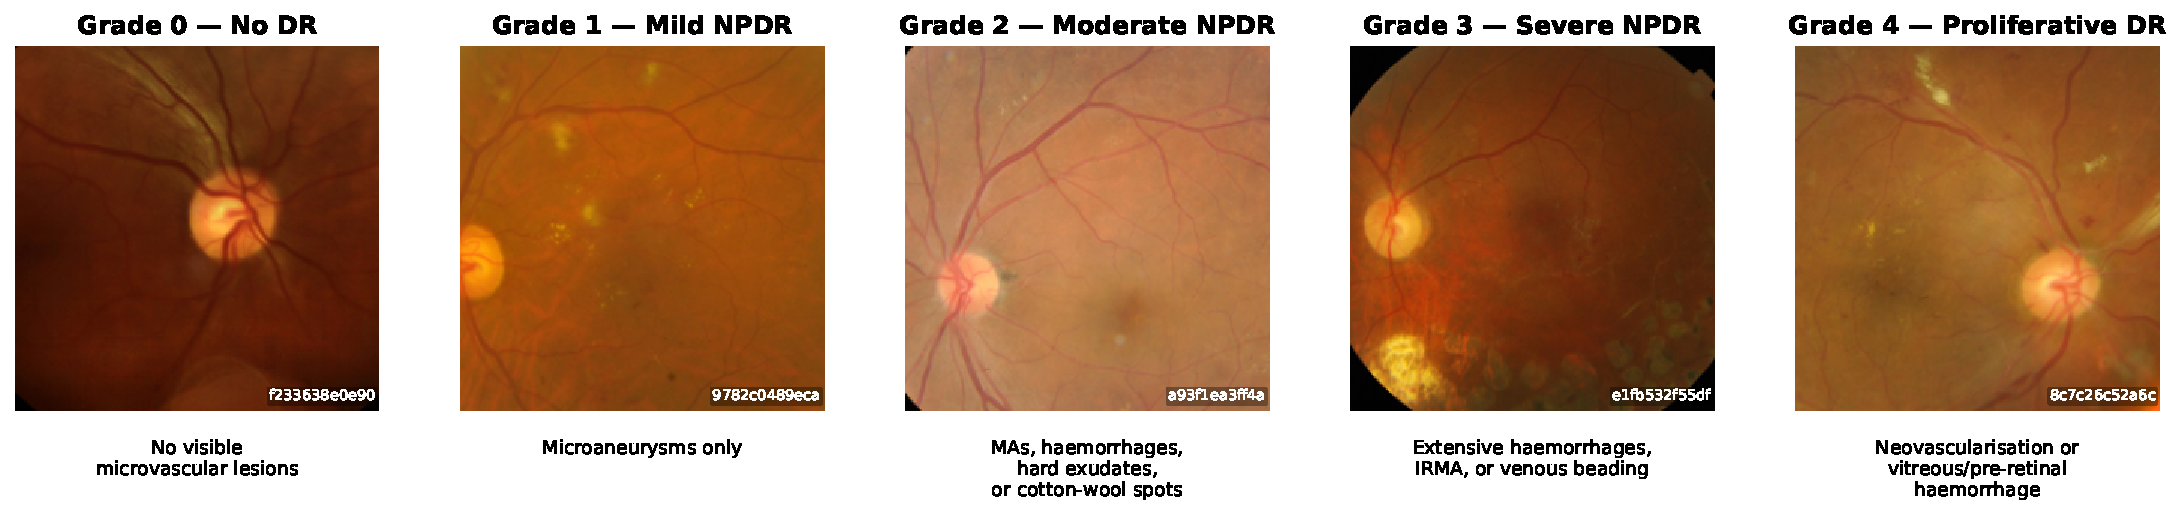
\includegraphics[width=\textwidth]{figs/fig_0_grade_samples.pdf}
    \caption{Representative APTOS-2019 samples across the five-point ICDR severity scale. Preprocessing follows the official RETFound evaluation transform (Resize-256 bicubic $\to$ CenterCrop-224 $\to$ ImageNet normalise). Clinical descriptors are standard ICDR definitions.}
    \label{fig:grades}
\end{figure*}

Recent DR-grading work has pushed on backbone scale (ViT-L ensembles, ConvNeXt-Base \cite{ref:uaorlqap}, MAFNet \cite{ref:mafnet}, Dual-SwinOrd \cite{ref:dualswinord}), on ordinal formulations (evidential \cite{ref:uaorlqap}), and on richer uncertainty layers (Bayesian heads, ensembles, evidential losses). This paper asks an orthogonal question. How much does the head actually matter once the backbone is frozen, and which uncertainty story survives an honest audit?

The headline finding from the head$\times$backbone grid is that the backbone dominates the head. Swapping the domain-specific RETFound for the generalist DINOv2 lifts grading agreement substantially on both datasets, an order of magnitude more than swapping the prediction head. On Messidor-2 with DINOv2 features the two heads are statistically indistinguishable. The advantage of capsule routing over the much simpler MLP+$K{-}1$ baseline is real but small on APTOS, and it vanishes once the backbone is strong enough. This narrows the case for domain-specific retinal pretraining and for capsule routing to a single regime, namely the 2023-generation RETFound-MAE backbone paired with a small ordinal head.

Why test capsules on an ordinal task at all? The a-priori argument is specific rather than generic. A DigitCaps layer represents each class by a \emph{vector} whose length is a bounded activation probability and whose orientation encodes instantiation parameters, and routing-by-agreement lets lower-level features vote for the classes they are consistent with \cite{ref:sabour}. For DR grading that maps onto something real: severity is signalled by a small number of spatially sparse lesions (microaneurysms, haemorrhages, neovascularisation), the ICDR grades are defined by which lesion types co-occur, and adjacent grades share most of their evidence. A part-whole voting mechanism with a length-as-probability output is therefore a plausible fit to an ordinal boundary, and existing capsule-DR work \cite{ref:gogulamudi,ref:gfcapsnet} asserts as much. What that work does not do is test the claim against a capacity-matched non-capsule control under the same ordinal decomposition, which is what makes the question open rather than settled. Our answer is that the hypothesis does not survive: the routing machinery buys $+0.007$ QWK on APTOS, nothing at all under a stronger backbone, and it is measurably worse on all three consistency axes we introduce below.

The capsule head is also commonly credited with a \emph{native} uncertainty signal, namely the margin between the top two capsule lengths. We find this signal essentially indistinguishable from the analogous top-2 margin of a plain MLP with sigmoid outputs, and the underlying capsule-length probabilities are systematically \emph{under}-confident: accuracy exceeds mean confidence in every equal-mass bin of all nine configurations, so the fitted temperature is below one and sharpens rather than softens. A single-parameter temperature rescaling closes most of the calibration gap, but on stricter scoring rules the MLP head still wins. The capsule margin behaves as a useful \emph{discriminative} score for ranking confident predictions. It is not a calibrated probability.

Split conformal prediction is the uncertainty layer that holds up. Asked for a $90\%$ confidence level, it returns a small \emph{set} of grades that contains the true grade $90\%$ of the time \emph{averaged over all patients}, and this guarantee holds on every cell of our grid. The catch is in the word \emph{averaged}. Under the standard scoring rules, that average is met by being very accurate on the no-DR majority while leaving the rare severe-DR cases under-covered, exactly the patients we can least afford to miss. A per-class quantile restores the guarantee \emph{separately for each grade} at a small cost in average set size. Conformal therefore turns frozen-feature DR grading into a probabilistically meaningful screening tool, with the caveat that per-grade reliability requires the per-class fix.

As a separate cross-dataset diagnostic, the APTOS-trained frozen head collapses to a near-constant Grade-0 predictor on Messidor-2 (99.4\% Grade-0 predictions; Zoellin et al.\ \cite{ref:zoellin} report frozen-RETFound Messidor QKappa of exactly $0.0$ in an independent setup). A standard post-hoc rescaling, using only the expected grade distribution on Messidor-2 with no true labels \cite{ref:saerens,ref:bbse}, lifts the model's agreement with clinicians from essentially zero to the \emph{fair} band of the standard kappa scale, still well below the threshold expected for clinical screening. We report this as a diagnostic that the failure is a threshold miscalibration rather than a feature-space collapse, not as a domain-adaptation contribution.

\noindent\textbf{Contributions.} The first two are methodological, and the rest is the evidence that motivates and evaluates them.
\begin{itemize}
    \item \emph{Rank-monotonicity as a constrained projection.} We replace the usual clip-and-renormalise repair of the $K{-}1$ chain rule with the exact Euclidean projection of the cumulative head vector onto the antitonic cone (Eq.~\eqref{eq:monotone}), solved in $O(K)$ by pool-adjacent-violators, followed by an exact cumulative-difference decode. The result is a valid distribution by construction, with no clipping and no renormalisation. It halves ECE on all nine cells at no parameter and no held-out split, and it exposes the fact that the previously reported renormalisation rate measured the decoding rather than the model.
    \item \emph{Ordinal contiguous prediction sets (OCP).} We give a conformal nonconformity score whose prediction sets are contiguous grade intervals by construction (Eq.~\eqref{eq:ocp}), obtained by accumulating probability mass in a mode-anchored nested-interval order instead of in descending-probability order. Because the score remains a fixed function of $(x,y)$, OCP inherits the split-conformal marginal-coverage guarantee unchanged. It removes the $0.6$--$12.8\%$ of ordinally incoherent sets that LAC, APS and RAPS emit, at a mean set-size cost of $0.04$ grades.
    \item \emph{Decomposing backbone, head, and tuning effects.} A fully-crossed head$\times$backbone ablation (capsule and MLP+$K{-}1$, RETFound and DINOv2) on APTOS and Messidor-2 at $3$ seeds $\times$ $5$ folds with paired Wilcoxon tests, extended to a four-tier fine-tuning comparison (frozen, LoRA, progressive unfreezing, full fine-tune) and an A100 complexity profile in FLOPs, peak memory and throughput.
    \item \emph{An honest audit of native capsule confidence.} Calibration across all nine cells with ECE, MCE, Brier, NLL, AURC and risk-at-coverage, against a temperature-scaling baseline; plus a loss$\times$head factorial that separates the contribution of the margin loss from that of the architecture.
    \item \emph{Clinical and cross-dataset evaluation.} Referable- and vision-threatening-DR sensitivity and specificity with bootstrap intervals against the NHS screening bar, and an APTOS$\to$Messidor-2 transfer study comparing feature-space alignment (CORAL) and label-shift correction (BBSE, EM) against rank calibration.
\end{itemize}
Code, configuration files, per-run metric summaries, the per-fold prediction arrays and an end-to-end regeneration script are available in the repository listed under Data Availability.

The remainder of this paper is organized as follows. Section~\ref{sec:related} reviews related work. Section~\ref{sec:method} describes the heads, backbones, and UQ layers, and Section~\ref{sec:setup} covers the datasets and protocol. Section~\ref{sec:results} reports the experiments, followed by a discussion in Section~\ref{sec:discussion}, limitations in Section~\ref{sec:limitations}, and conclusions in Section~\ref{sec:conclusion}. Negative ablations are collected in Appendix~\ref{sec:negatives}.

\section{Related Work}
\label{sec:related}

\subsection{Ordinal DR grading}
Niu et al.\ \cite{ref:niu} introduced the $K{-}1$ binary decomposition. Rank consistency across the $K{-}1$ thresholds is not guaranteed by that formulation, and two lines of work address it directly: CORAL \cite{ref:coral} enforces it architecturally by sharing a single weight vector across thresholds, and CORN \cite{ref:corn} obtains it instead through conditional training subsets and a chain-rule factorisation, without the weight-sharing constraint. Our projection of Eq.~\eqref{eq:monotone} is a third, post-hoc route to the same property: it leaves training untouched and enforces monotonicity at decode time, which lets us quantify how often the unconstrained heads actually violate it. The model trains $K{-}1$ binary classifiers, each answering whether the rank exceeds threshold $k$, and decodes the rank as $1 + \sum_k \mathbf{1}[f_k(x){>}0.5]$. Recent DR-specific extensions vary the backbone and the loss. El Bellaj et al.\ \cite{ref:uaorlqap} pair a ConvNeXt-Base with an evidential Dirichlet head. MAFNet \cite{ref:mafnet} is a multi-scale adaptive fine-grained network. Dual-SwinOrd \cite{ref:dualswinord} pairs a Swin Transformer backbone with a PubMedCLIP-guided semantic prior and dual classification and ordinal-regression heads. Our setup is deliberately simpler so the backbone, head, and uncertainty-layer effects can be cleanly separated.

\subsection{Foundation models for retinal imaging}
RETFound \cite{ref:retfound} is a ViT-L masked autoencoder pretrained on $904$k CFPs and $736$k OCT scans. DINOv2 \cite{ref:dinov2} is a general-purpose self-supervised ViT trained on LVD-142M without retinal specialisation. A recent head-to-head evaluation on retinal downstream tasks \cite{ref:dinov2_vs_retfound} reports that DINOv2 outperforms RETFound on ocular-disease detection (including DR) while RETFound retains an edge on systemic-disease incidence prediction. Poyrazer et al.\ \cite{ref:dinov2_vs_retfound} benchmark frozen-encoder cross-dataset transfer for DR with calibration as a co-primary endpoint, and Isztl et al.\ \cite{ref:zoellin} evaluate the parameter-cost of specialised retinal backbones across multiple retinal imaging tasks. The LoRA adapter \cite{ref:lora} is used as our lightweight fine-tuning counterpoint.

\subsection{Capsule networks for DR}
Sabour, Frosst, and Hinton \cite{ref:sabour} introduced capsules with routing-by-agreement and a margin loss. On retinal fundus photography, Gogulamudi et al.\ \cite{ref:gogulamudi} propose a non-uniform squash on a custom 7-class dataset, and Lei et al.\ \cite{ref:gfcapsnet} fuse a GNN layer into the PrimaryCaps$\to$DigitCaps transformation. Neither reports QWK, cross-dataset evaluation, or calibration, which is precisely the evidence needed to judge whether routing earns its place in an ordinal grader.

\subsection{Calibration and conformal UQ in medical imaging}
Two frameworks are standard for attaching uncertainty to neural-network classifiers. Expected Calibration Error (ECE) \cite{ref:guo_calibration} measures the average gap between a model's reported confidence and its empirical accuracy across equal-mass confidence bins, and indicates whether the reported probabilities can be trusted as probabilities. Split conformal prediction \cite{ref:vovk_conformal} operates differently, returning a small set of candidate labels per input with a distribution-free marginal-coverage guarantee that depends only on exchangeability between the calibration and test data, not on whether the underlying probabilities are well-calibrated. For multi-class problems, LAC \cite{ref:sadinle} and APS \cite{ref:romano} are the canonical nonconformity scores. Shi et al.\ \cite{ref:rank_conformal} address the class-conditional coverage gap that LAC and APS exhibit, by augmenting label ranks; a companion line of work targets the same gap under severe class imbalance by restricting to top-$k$ label sets \cite{ref:kccp}. Both keep the label set unordered, so neither yields contiguous grade intervals.

\section{Materials and Methods}
\label{sec:method}

\subsection{Backbones}
We evaluate two frozen ViT-L-scale backbones at 224$\times$224 input resolution. RETFound ViT-L/16 \cite{ref:retfound} is pretrained on retinal CFPs. DINOv2 ViT-L/14 \cite{ref:dinov2} is pretrained on 142M natural images with no retinal specialisation. Both produce a 1024-dim CLS token; the preprocessing pipeline (Resize-256 bicubic $\to$ CenterCrop-224 $\to$ ImageNet normalise) is identical for both backbones, so the only changing variable is the backbone weights. A LoRA rank-8 variant of RETFound \cite{ref:lora} is added as a fine-tuning counterpoint (see Section~\ref{sec:lora}).

\subsection{Ordinal heads on frozen features}
We compare two head architectures, both using Niu's $K{-}1$ binary decomposition and an identical Sabour-style margin loss with $m^+ = 0.9$, $m^- = 0.1$, $\lambda = 0.5$ \cite{ref:sabour}. Head A (\textit{Ordinal CapsNet}) is a PrimaryCaps layer (32 capsules of dim 8) followed by four independent DigitCaps heads (2 capsules of dim 16, 3 routing iterations per head), one per ordinal threshold. Head B (\textit{MLP + $K{-}1$ sigmoid}) is a plain MLP ($1024 \to 256 \to 256 \to \mathbb{R}^{K-1}$) with four independent sigmoid output heads. Head B is a direct no-capsule comparator with no routing and no capsule nonlinearity, using the same loss and the same decomposition. Trainable parameter counts are $\approx$295K (CapsNet) and $\approx$329K (MLP-K1) respectively, capacity-matched within $10\%$ so the ablation does not confound capacity with architecture.

\subsection{LoRA variant}
\label{sec:lora}
In the LoRA configuration we unfreeze nothing in RETFound but inject rank-8 adapters into the fused \texttt{attn.qkv} projection of every ViT-L block (24 blocks). Scaling $\alpha = 16$, dropout $0.05$. The optimiser uses two groups, with LoRA learning rate $10^{-4}$ and head learning rate $10^{-3}$. Total trainable count is $\approx$1.08M ($0.35\%$ of the backbone's 307M).

\subsection{Decoding and chain-rule probability}
At inference, each head produces a probability $\hat{p}_k = P(y{>}k\,|\,x)$ from the length of its positive capsule (CapsNet) or its sigmoid output (MLP-K1). The predicted grade is
\begin{equation}
    \hat{y} \;=\; \sum_{k=0}^{K-2} \mathbf{1}\bigl[\hat{p}_k > 0.5\bigr].
    \label{eq:predict}
\end{equation}
We also compute a 5-class probability vector from the $K{-}1$ head outputs. The submitted form of this paper used the product decoding $P(y{=}k) = \hat{p}_{k-1}(1{-}\hat{p}_k)$, clipped at zero and renormalised. That repair is unsatisfactory in two ways, and we replace it below.

\subsection{Rank-monotonicity as a constrained projection}
\label{sec:monotone}
The product decoding does not define a distribution even when the heads are perfectly rank-consistent: for $\hat{p} = (0.5, 0.4, 0.3, 0.2)$ it sums to $1.52$. Renormalisation therefore fires on essentially every sample, and the resulting rate measures the decoding, not the model. Separately, clipping negative entries is not the solution of any stated optimisation problem.

We fix both by imposing rank-monotonicity where it belongs, on the \emph{cumulative} probabilities, before decoding. Given raw head outputs $\hat{p} \in [0,1]^{K-1}$ we solve
\begin{equation}
    \tilde{p} \;=\; \arg\min_{q}\; \tfrac{1}{2}\lVert q - \hat{p} \rVert_2^2
    \quad \text{s.t.} \quad 1 \geq q_1 \geq q_2 \geq \cdots \geq q_{K-1} \geq 0,
    \label{eq:monotone}
\end{equation}
the Euclidean projection onto the intersection of the antitonic cone with the unit box. This is antitonic regression and the Pool-Adjacent-Violators algorithm solves it exactly in $O(K)$; no iterative solver is needed, and since $\hat{p}$ already lies in $[0,1]^{K-1}$ and PAV returns weighted averages of its inputs, the box constraints are satisfied automatically. Decoding then uses exact cumulative differences,
\begin{equation}
    P(y{=}0) = 1 - \tilde{p}_1, \quad
    P(y{=}k) = \tilde{p}_k - \tilde{p}_{k+1}, \quad
    P(y{=}K{-}1) = \tilde{p}_{K-1},
    \label{eq:decode}
\end{equation}
which is non-negative and sums to exactly one by construction. No clipping and no renormalisation ever run. All UQ metrics below (ECE, AURC, conformal) operate on this probability basis.

\subsection{Uncertainty quantification}
\label{sec:uq-method}
We evaluate the following UQ views on the same chain-rule probabilities.

\emph{Calibration.} Expected Calibration Error with 10 equal-mass bins on the confidence signal $c_i = P(y = \hat{y}_i)$ (i.e., calibration of the model's confidence in its own K-1 decision). We also report MCE (worst-bin gap).

\emph{Selective prediction.} Area Under the Risk--Coverage curve (AURC) and its excess over the oracle. We compare two confidence signals: (i) $\max_k P(y{=}k)$ and (ii) the prediction margin $1 - (p_{\text{top}_1} - p_{\text{top}_2})$, which has been highlighted in recent capsule-UQ work.

\emph{Conformal prediction.} Split conformal with four nonconformity scores: LAC \cite{ref:sadinle} (nonconformity $= 1 - P(y_{\text{true}})$), APS \cite{ref:romano} (cumulative descending probability), RAPS \cite{ref:raps}, and the ordinal-contiguous score OCP introduced below; we additionally report Mondrian \cite{ref:mondrian} per-class quantiles. Calibration and test halves are drawn by a 50:50 random split, averaged over five split seeds. Conformal requires only exchangeability, not calibration, so it gives a guarantee that survives the ECE problems documented in Section~\ref{sec:calibration}.

\subsection{Ordinal contiguous prediction sets (OCP)}
\label{sec:ocp}
LAC, APS and RAPS treat the $K$ grades as an unordered label set, so their prediction sets may skip an intermediate grade. A set such as $\{0,3\}$ asserts that the eye is either healthy or severe but definitely not moderate, which is incoherent on an ordinal scale and unusable for triage.

We obtain contiguity by construction rather than by post-hoc repair. For a sample $x$ let $m = \arg\max_k P(y{=}k)$ and define a nested family of \emph{intervals} $I_1 \subset I_2 \subset \cdots \subset I_K$ by $I_1 = \{m\}$, absorbing at each step whichever neighbour of the current interval carries more probability mass (ties break toward the lower grade, the safety-conservative direction for screening). Writing $j^\star(y) = \min\{j : y \in I_j\}$, the nonconformity score is
\begin{equation}
    s(x,y) \;=\; \sum_{c \in I_{j^\star(y)}} P(y{=}c) \;-\; u \cdot P(y{=}y),
    \label{eq:ocp}
\end{equation}
with $u \sim \mathcal{U}[0,1]$ the standard randomised tie-breaker \cite{ref:romano}. The prediction set is the corresponding $\hat{q}$ sublevel set, which is an interval $[a,b]$ because the $I_j$ are.

OCP is exactly APS with the descending-probability accumulation order replaced by this ordinal nesting order. The score therefore remains a fixed measurable function of $(x,y)$, evaluated identically on calibration and test points, so the split-conformal exchangeability argument is untouched and OCP inherits the same distribution-free $1-\alpha$ marginal coverage guarantee. Contiguity costs nothing in validity; Section~\ref{sec:conformal-results} quantifies what it costs in set size.

\section{Experimental Setup}
\label{sec:setup}

\subsection{Datasets}
\textbf{APTOS-2019} \cite{ref:aptos} contains 3{,}662 colour fundus photographs (CFPs) with 5-class ICDR severity labels. \textbf{Messidor-2} \cite{ref:messidor2,ref:abramoff} is distributed as 1{,}748 images, of which 1{,}744 carry an adjudicated 5-class grade; the 4 images marked ungradable by the adjudication protocol are excluded, since a severity label does not exist for them. We do not perform any additional automated quality filtering, so every gradable image is retained regardless of illumination or focus, and no image is discarded on the basis of model confidence. APTOS and IDRiD are distributed fully graded and are used in their entirety. \textbf{IDRiD} \cite{ref:idrid} contains 413 training and 103 official-test images with 5-class labels.

\subsection{Metrics}
\label{sec:metrics}
We report metrics in three families.

\textit{Grading agreement.} Quadratic Weighted Kappa (QWK) is the primary metric. It measures agreement with the clinician label on the ordinal ICDR scale and penalises distant errors more than adjacent ones. QWK $1.0$ is perfect agreement and $0$ is chance. Following the standard Landis and Koch interpretation \cite{ref:landiskoch}, we read $\geq 0.61$ as substantial, $0.41$ to $0.60$ as moderate, $0.21$ to $0.40$ as fair, and below $0.20$ as slight or worse. We also report top-1 accuracy, macro-F1, and mean absolute error in grade units.

\textit{Probability calibration.} Expected Calibration Error (ECE) bins predictions by their confidence and reports the average gap between confidence and accuracy. Maximum Calibration Error (MCE) reports the worst single bin. Brier score and negative log-likelihood (NLL) are proper scoring rules that combine calibration and discrimination. Lower is better for all four.

\textit{Selective prediction and prediction sets.} Area Under the Risk-Coverage curve (AURC) measures how cleanly a confidence signal can rank correct against incorrect predictions for selective prediction. For conformal prediction we report marginal coverage (the fraction of test samples whose true grade lies in the predicted set), worst-class coverage (the same fraction restricted to the rarest grade), and mean prediction-set size at confidence level $1 - \alpha$ for $\alpha \in \{0.10, 0.05\}$.

\subsection{Protocol}
Every row of the APTOS ablation is 3 seeds $\times$ 5 folds (seeds $\{42, 123, 456\}$). The LoRA fine-tune reported in Section~\ref{sec:aptos} uses the same protocol. On APTOS we set aside a class-stratified $10\%$ holdout and run stratified 5-fold CV on the remaining $90\%$. On Messidor-2 we run stratified 5-fold within-dataset and additionally report APTOS$\to$Messidor-2 cross-dataset transfer with no Messidor-2 training. IDRiD is used for within-dataset evaluation and APTOS$\to$IDRiD cross-dataset transfer on the RETFound backbone only. Data splits are fixed across seeds by \texttt{cfg.data.seed}, so only the model-init RNG varies. Early-stopping patience is 30 epochs on validation QWK (8 for LoRA, which converges in roughly half the budget). The optimiser is AdamW with weight decay $10^{-4}$.

\emph{Data augmentation.} None is applied. In the frozen-feature tiers the backbone is evaluated once per image under the deterministic RETFound evaluation transform and its CLS token is cached, so augmentation would have no effect unless the cache were regenerated per epoch; holding the features fixed is what makes the head comparison exactly controlled. For the LoRA and fine-tuning tiers, where the backbone does see gradients, augmentation would have been possible and we deliberately omitted it so that every tier in Table~\ref{tab:finetune} differs only in which parameters are trainable. This is a limitation rather than a design virtue: Ahamed et al. \cite{ref:dr_conformal} show that augmentation choices interact non-trivially with conformal coverage on DR grading, so an augmented variant is a natural extension.

\emph{Calibration/test construction and exchangeability.} All conformal results split a pooled prediction set 50:50 at random into calibration and test halves, averaged over five split seeds. Two caveats about the exchangeability this relies on. First, the pool is formed by concatenating out-of-fold predictions across 5 folds and 3 model seeds, so each image contributes 3 rows (one per seed) produced by different models. These rows are not independent, which inflates the effective sample size relative to the nominal $N = 9{,}885$. Second, predictions from different folds come from different fitted heads, so the pooled sequence is exchangeable only under the additional assumption that the fold-wise models are themselves exchangeable. Neither caveat affects the observed coverage, which we verify empirically holds within $\pm 0.01$ of target in every configuration, but both mean the finite-sample guarantee should be read as approximate. A strictly exchangeable alternative is to calibrate within a single fold of a single seed, at $1/15$ of the pooled sample size ($N = 659$). We ran it: coverage is $0.9447 \pm 0.0180$ against $0.9505 \pm 0.0039$ for the pooled set, a difference of $0.0058$ that sits inside one standard deviation of the strict estimate, with mean set size $1.909$ versus $1.934$. Pooling therefore buys a much tighter coverage estimate without measurably biasing it.

\section{Results}
\label{sec:results}

\subsection{APTOS ablation}
\label{sec:aptos}

Table~\ref{tab:aptos} reports the head-level ablation on frozen RETFound features. Every row is 3 seeds $\times$ 5-fold CV.

\begin{table*}[!t]
    \caption{APTOS-2019 head ablation on frozen RETFound ViT-L/16 features. Every row is 3 seeds $\times$ 5-fold CV (seeds 42/123/456). QWK, Accuracy, and Macro-F1: higher is better. MAE: lower is better. Best value per column among the seven primary heads in \textbf{bold}; rows marked $\dag$ are loss and squash variants of row 6 and are excluded from that comparison.}
    \label{tab:aptos}
    \centering
    \footnotesize
    \begin{tabular}{@{}clcccc@{}}
        \toprule
        \# & Model                                       & QWK                          & Accuracy                     & Macro-F1                     & MAE                        \\
        \midrule
        1  & Linear + CE                                 & $0.8389 \pm 0.0122$           & $0.7971 \pm 0.0038$           & $0.6011 \pm 0.0144$           & $0.291 \pm 0.011$ \\
        2  & MLP + CE                                    & $0.8755 \pm 0.0014$           & $\mathbf{0.8091 \pm 0.0021}$ & $\mathbf{0.6325 \pm 0.0067}$ & $0.258 \pm 0.002$ \\
        3  & MLP + MSE                                   & $0.8813 \pm 0.0012$           & $0.7438 \pm 0.0113$           & $0.5433 \pm 0.0051$           & $0.295 \pm 0.011$ \\
        4  & MLP + Weighted CE                           & $0.8638 \pm 0.0021$           & $0.7796 \pm 0.0048$           & $0.6262 \pm 0.0074$           & $0.291 \pm 0.006$ \\
        5  & Vanilla CapsNet                             & $0.8696 \pm 0.0026$           & $0.8061 \pm 0.0046$           & $0.6301 \pm 0.0044$           & $0.263 \pm 0.003$ \\
        6  & Ordinal CapsNet                             & $\mathbf{0.8923 \pm 0.0002}$ & $0.7935 \pm 0.0075$           & $0.6259 \pm 0.0089$           & $\mathbf{0.256 \pm 0.006}$ \\
        7  & MLP + $K{-}1$ sigmoid                       & $0.8849 \pm 0.0015$           & $0.7976 \pm 0.0088$           & $0.6235 \pm 0.0106$           & $0.258 \pm 0.010$ \\
        8  & \quad Ordinal + Asymmetric loss$^{\dag}$    & $0.8924 \pm 0.0002$  & $0.7923 \pm 0.0041$           & $0.6247 \pm 0.0043$           & $0.257 \pm 0.003$ \\
        9  & \quad Ordinal + KC Loss$^{\dag}$            & $0.8916 \pm 0.0005$           & $0.7840 \pm 0.0027$           & $0.6126 \pm 0.0045$           & $0.261 \pm 0.002$ \\
        10 & \quad Ordinal + Non-uniform squash$^{\dag}$ & $0.8890 \pm 0.0001$           & $0.7893 \pm 0.0014$           & $0.6122 \pm 0.0034$           & $0.262 \pm 0.001$ \\
        \bottomrule
        \multicolumn{6}{l}{\scriptsize $^{\dag}$ Negative-result ablations. See Appendix~\ref{sec:negatives}.}
    \end{tabular}
\end{table*}

The $K{-}1$ ordinal decomposition is the larger head-level lever; capsule routing is a smaller second-order improvement on top of it. Moving from plain MLP+CE to MLP+$K{-}1$ lifts QWK by $+0.0094$. Adding capsule routing on top of MLP+$K{-}1$, which gives our Ordinal CapsNet head, lifts QWK by a further $+0.0074$. Both contributions are outside seed noise (across-seed std $\leq 0.0015$ on each row, against contribution sizes an order of magnitude larger).

\textit{What fine-tuning buys.} For comparison, fine-tuning the RETFound backbone with LoRA r=8 (1.08M trainable parameters injected into the attention projections, $\approx$16h per seed on MPS) and keeping the same Ordinal CapsNet head reaches QWK $0.9143 \pm 0.0006$ on the same 3-seed 5-fold protocol, an additional $+0.022$ QWK over the same head on frozen RETFound features. The remainder of this paper analyses frozen-feature configurations on consumer hardware; we report LoRA only as a compute-tier anchor.

\subsection{Head\,$\times$\,Backbone 2$\times$2 ablation}
\label{sec:head-backbone}

Table~\ref{tab:head_backbone} is the fully crossed ablation on APTOS and Messidor-2. The single-variable change column (backbone) yields a substantially larger effect than the orthogonal single-variable change (head) on both datasets.

\begin{table*}[!t]
    \caption{Head $\times$ backbone ablation. APTOS rows are 3 seeds $\times$ 5-fold CV; Messidor-2 rows are 5-fold CV on the 1{,}744 gradable images. All cells share preprocessing, decomposition and loss.}
    \label{tab:head_backbone}
    \centering
    \footnotesize
    \begin{tabular}{@{}lcccccc@{}}
        \toprule
        \textbf{Head}   & \multicolumn{3}{c}{\textbf{APTOS-2019 QWK}} & \multicolumn{3}{c}{\textbf{Messidor-2 within QWK}}                                                                                     \\
        \cmidrule(r){2-4}\cmidrule(l){5-7}
                        & RETFound                                    & DINOv2                                             & $\Delta$ backbone & RETFound            & DINOv2              & $\Delta$ backbone \\
        \midrule
        Ordinal CapsNet & $0.8923 \pm 0.0002$ & $0.9074 \pm 0.0029$ & $+0.0152$         & $0.6021 \pm 0.0454$ & $0.7586 \pm 0.0187$ & $+0.1565$         \\
        MLP + K-1 sig   & $0.8849 \pm 0.0015$ & $0.9041 \pm 0.0007$ & $+0.0192$         & $0.5900 \pm 0.0312$ & $0.7587 \pm 0.0209$ & $+0.1687$         \\
        $\Delta$ head   & $+0.0073$           & $+0.0033$           & ---               & $+0.0121$           & $-0.0002$           & ---               \\
        \bottomrule
    \end{tabular}
\end{table*}

DINOv2 beats RETFound at frozen-feature DR grading cleanly on both datasets and both heads. On Messidor-2 the backbone effect ($+0.157$ to $+0.169$ QWK) is roughly $13\times$ the head effect ($+0.012$ QWK at RETFound and $-0.0002$ at DINOv2), and under the stronger DINOv2 backbone the head effect vanishes entirely: the two heads are statistically indistinguishable (QWK $0.7586$ vs.\ $0.7587$, Wilcoxon $p = 1.00$, capsule ahead on 3 of 5 folds). The head is a smaller lever than the backbone in this regime, and once the backbone is strong enough the capsule machinery stops contributing at all.

\subsection{Calibration analysis}
\label{sec:calibration}

Table~\ref{tab:calibration} summarises the calibration and selective-prediction metrics across all nine configurations. Fig.~\ref{fig:reliability_aptos} shows reliability diagrams for the APTOS head$\times$backbone $2{\times}2$.

\begin{table*}[!t]
    \caption{Calibration and selective prediction across the head$\times$backbone grid. Lower is better in all four UQ columns. Renorm reflects the product decoding rather than ordinal consistency (Section~\ref{sec:monotone}). \textbf{Bold} = best among frozen-feature rows; LoRA is a compute-tier anchor.}
    \label{tab:calibration}
    \centering
    \footnotesize
    \begin{tabular}{@{}llcccccc@{}}
        \toprule
        Dataset    & Model                             & Acc            & ECE            & MCE            & AURC (max-p)   & AURC (margin)  & Renorm \\
        \midrule
        APTOS      & RETFound $\times$ Ordinal CapsNet & 0.794           & 0.143           & 0.225           & 0.0591          & 0.0596          & 100\%  \\
                   & RETFound $\times$ MLP-K1          & 0.798           & \textbf{0.098}  & 0.175           & 0.0617          & 0.0601          & 86\%   \\
                   & DINOv2 $\times$ Ordinal CapsNet   & 0.804           & 0.120           & 0.191           & \textbf{0.0497} & 0.0495          & 100\%  \\
                   & DINOv2 $\times$ MLP-K1            & \textbf{0.809}  & 0.103           & \textbf{0.169}  & 0.0500          & \textbf{0.0485} & 100\%  \\
                   & RETFound $\times$ Ordinal + LoRA  & 0.824           & 0.131           & 0.181           & 0.0485          & 0.0477          & 100\%  \\
        \midrule
        Messidor-2 & RETFound $\times$ Ordinal CapsNet & 0.577           & 0.103           & 0.188           & 0.2380          & 0.2394          & 100\%  \\
                   & RETFound $\times$ MLP-K1          & 0.584           & 0.083           & 0.154           & 0.2353          & 0.2360          & 100\%  \\
                   & DINOv2 $\times$ Ordinal CapsNet   & \textbf{0.690}  & 0.121           & 0.194           & \textbf{0.1795} & \textbf{0.1786} & 100\%  \\
                   & DINOv2 $\times$ MLP-K1            & 0.685           & \textbf{0.077}  & \textbf{0.132}  & 0.1882          & 0.1839          & 100\%  \\
        \bottomrule
    \end{tabular}
\end{table*}

\begin{figure}[!t]
    \centering
    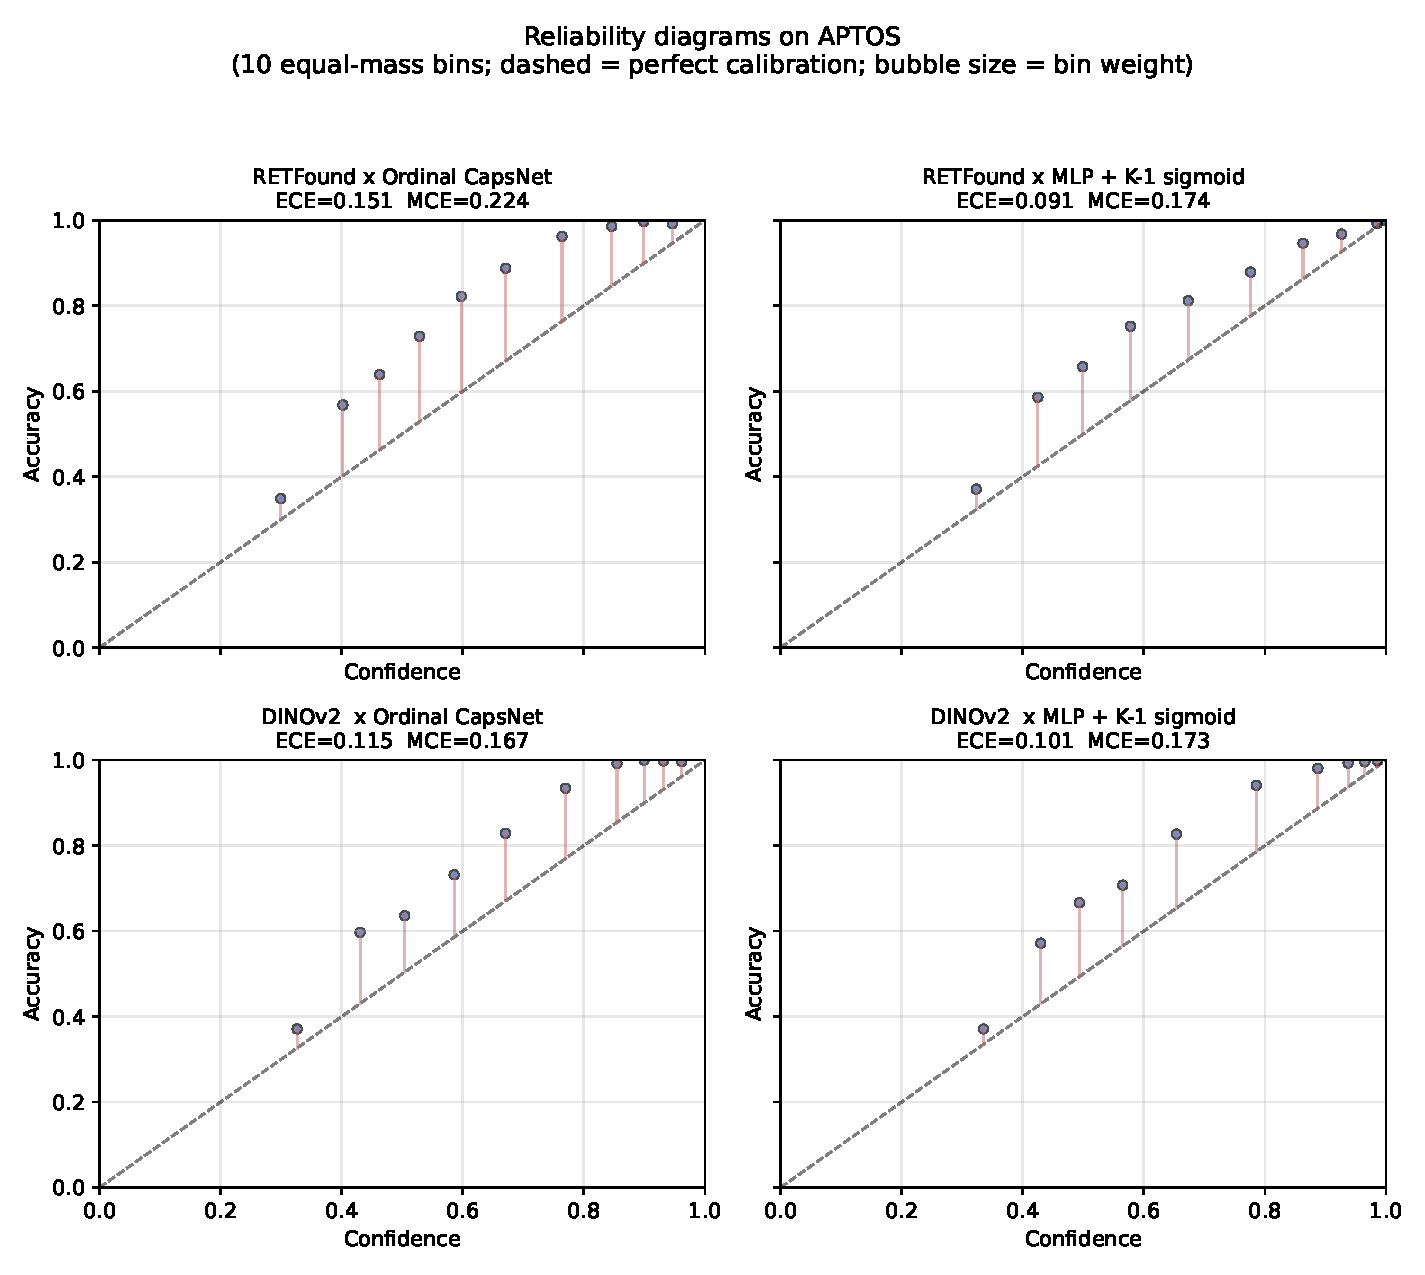
\includegraphics[width=\columnwidth]{figs/fig_reliability_aptos.pdf}
    \caption{APTOS reliability diagrams for the four head$\times$backbone cells. Bubble size is bin weight. A perfectly calibrated head would lie on the dashed diagonal. Every cell sits above the diagonal: these heads are under-confident, and the capsule heads (top-left, bottom-left) more severely so than the MLP-K1 sigmoid head.}
    \label{fig:reliability_aptos}
\end{figure}

\begin{figure}[!t]
    \centering
    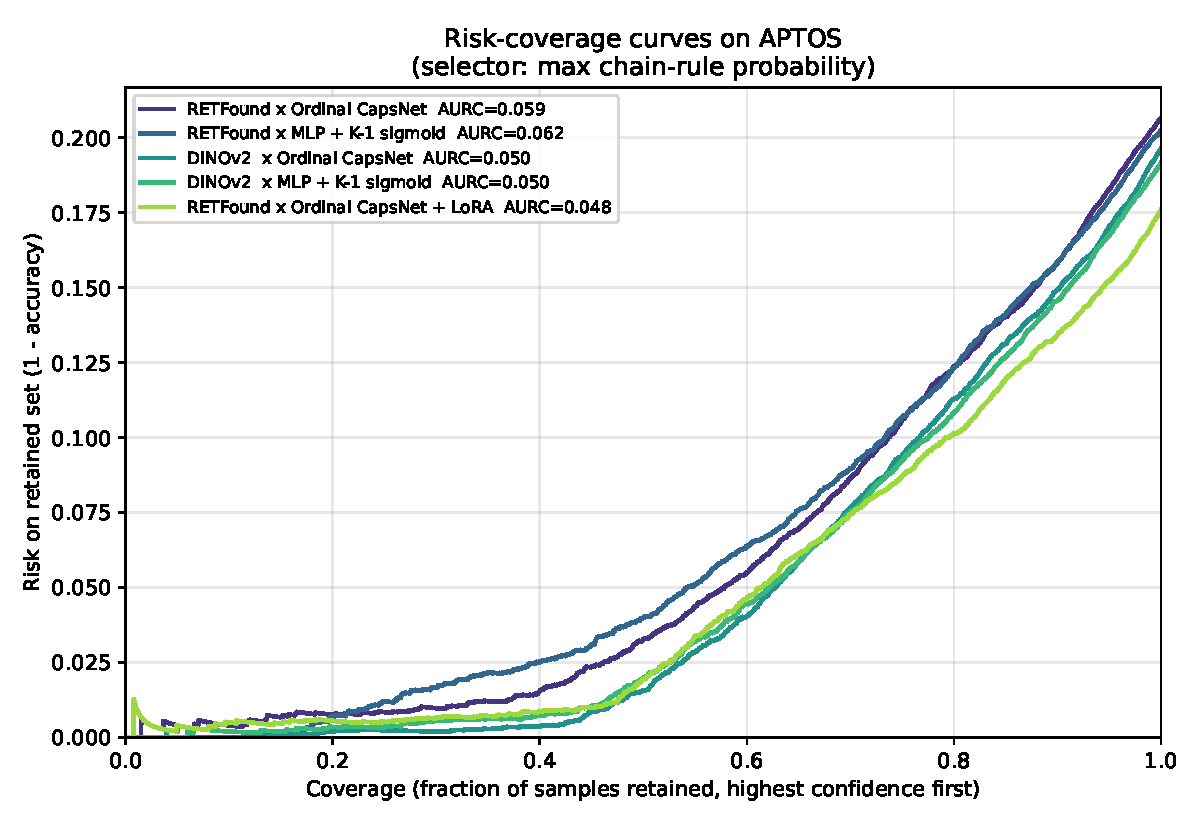
\includegraphics[width=\columnwidth]{figs/fig_risk_coverage_aptos.pdf}
    \caption{APTOS risk--coverage curves (max-p selector). Lower is better. DINOv2 curves dominate RETFound curves; within each backbone, capsule and MLP heads are near-identical.}
    \label{fig:risk_coverage_aptos}
\end{figure}

The capsule head is worse-calibrated than the MLP-K1 sigmoid head in all four head$\times$backbone cells (APTOS ECE $0.143$ vs.\ $0.098$ at RETFound and $0.120$ vs.\ $0.102$ at DINOv2; Messidor-2 $0.103$ vs.\ $0.083$ and $0.121$ vs.\ $0.077$). The mechanistic reason is that the Sabour margin loss \cite{ref:sabour} is a geometric clamping objective, not a proper scoring rule. It pushes the positive-capsule length above $m^+=0.9$ and the negative below $m^-=0.1$ regardless of the empirical base rate, whereas cross-entropy and log-loss on sigmoid outputs are minimised only when the predicted probability matches the true posterior. The non-linear squash further compresses vector magnitudes in a class-symmetric way that decouples length from observed frequency. The capsule's high ECE is thus not a training artefact but a direct consequence of the loss. LoRA inherits the miscalibration (ECE $0.141$) while improving discrimination.

Temperature scaling \cite{ref:guo_calibration} recovers most of the ECE gap (Table~\ref{tab:calibration_ts}). On APTOS the post-TS ECE is in the $0.011$ to $0.017$ range for every configuration, with fitted $T < 1$ everywhere. TS is less effective under domain shift (Messidor-2 post-TS ECE $0.022$ to $0.048$). It does not, however, close the Brier and NLL gap. Even post-TS, MLP-K1 ends up with the lowest Brier on Messidor-2 ($0.420$ vs.\ $0.432$ for DINOv2 $\times$ Ordinal CapsNet). The capsule head's probability estimates are recoverable as calibrated scalars via TS, but their joint distribution over classes remains inferior to a plainer head.

The capsule \emph{prediction margin} is also a valid selective-prediction signal but not a unique one. Fig.~\ref{fig:risk_coverage_aptos} shows the corresponding risk--coverage curves: within each backbone the capsule and MLP curves are visually indistinguishable, while the DINOv2 curves dominate the RETFound ones. AURC (margin) and AURC (max-p) agree within $\pm 0.004$ on every cell, and a vanilla MLP-K1 top-2 margin matches both. The UQ value attributed in prior work to the capsule nonlinearity is duplicated by the chain-rule 5-class probabilities of any $K{-}1$ head, capsule or otherwise.

\begin{table*}[!t]
    \caption{Temperature scaling on the chain-rule probabilities. $T$ is fitted on a random 50\% split by minimising NLL and evaluated on the other half. $T < 1$ sharpens the decoded distribution, which is the correction for under-confidence. Lower is better throughout.}
    \label{tab:calibration_ts}
    \centering
    \footnotesize
    \begin{tabular}{@{}llccccc@{}}
        \toprule
        Dataset & Model                    & T    & ECE$^{\text{pre}}$ & ECE$^{\text{post}}$ & Brier$^{\text{post}}$ & NLL$^{\text{post}}$ \\
        \midrule
        APTOS   & RET$\times$Ord.\ Caps    & 0.58                & 0.137               & 0.012               & 0.286               & 0.573 \\
                & RET$\times$MLP-K1        & 0.66                & \textbf{0.094}      & 0.014               & 0.286               & 0.570 \\
                & DINO$\times$Ord.\ Caps   & 0.60                & 0.120               & 0.016               & 0.268               & 0.523 \\
                & DINO$\times$MLP-K1       & 0.61                & 0.102               & \textbf{0.011}      & \textbf{0.263}      & \textbf{0.503} \\
                & RET$\times$Ord.\ +\,LoRA & 0.62                & 0.132               & 0.017               & 0.254               & 0.509 \\
        \midrule
        Mess-2  & RET$\times$Ord.\ Caps    & 0.67                & 0.109               & 0.048               & 0.522               & 0.989 \\
                & RET$\times$MLP-K1        & 0.75                & 0.081               & 0.028               & 0.516               & 0.995 \\
                & DINO$\times$Ord.\ Caps   & 0.66                & 0.120               & 0.037               & 0.432               & 0.808 \\
                & DINO$\times$MLP-K1       & 0.77                & \textbf{0.076}      & \textbf{0.022}      & \textbf{0.420}      & \textbf{0.781} \\
        \bottomrule
    \end{tabular}
\end{table*}

\subsection{Conformal prediction}
\label{sec:conformal-results}
\label{sec:conformal}

Calibration is miscalibrated because the margin loss does not encourage it; conformal prediction sidesteps the problem by producing coverage guarantees that depend only on exchangeability, not on probability calibration. Table~\ref{tab:conformal} shows marginal coverage and average set size at $\alpha = 0.10$ for all nine configurations, averaged over five random cal/test splits.

\begin{table*}[!t]
    \caption{Split conformal prediction at $\alpha = 0.10$ (target coverage 90\%), averaged over five random 50:50 calibration/test splits. Smaller $|S|$ is more informative at equal coverage. \textbf{Bold} = best among frozen-feature rows.}
    \label{tab:conformal}
    \centering
    \footnotesize
    \begin{tabular}{@{}llcc@{}}
        \toprule
        Dataset    & Model                             & Marginal cov.     & Mean $|S|$               \\
        \midrule
        APTOS      & RETFound $\times$ Ordinal CapsNet & $0.903 \pm 0.006$ & $1.38 \pm 0.02$           \\
                   & RETFound $\times$ MLP-K1          & $0.902 \pm 0.006$ & $1.37 \pm 0.02$           \\
                   & DINOv2 $\times$ Ordinal CapsNet   & $0.906 \pm 0.003$ & $1.32 \pm 0.01$           \\
                   & DINOv2 $\times$ MLP-K1            & $0.900 \pm 0.002$ & $\mathbf{1.29 \pm 0.01}$  \\
                   & RETFound $\times$ Ordinal + LoRA  & $0.903 \pm 0.007$ & $1.28 \pm 0.02$           \\
        \midrule
        Messidor-2 & RETFound $\times$ Ordinal CapsNet & $0.909 \pm 0.012$ & $2.33 \pm 0.05$           \\
                   & RETFound $\times$ MLP-K1          & $0.904 \pm 0.012$ & $2.30 \pm 0.05$           \\
                   & DINOv2 $\times$ Ordinal CapsNet   & $0.903 \pm 0.008$ & $1.85 \pm 0.03$           \\
                   & DINOv2 $\times$ MLP-K1            & $0.903 \pm 0.006$ & $\mathbf{1.83 \pm 0.02}$  \\
        \bottomrule
    \end{tabular}
\end{table*}

Every configuration hits the $90\%$ coverage target (observed range $90.0\%$ to $90.9\%$), as expected from the exchangeability guarantee of split CP \cite{ref:vovk_conformal}; what we are empirically verifying is that the guarantee holds on our data pipeline and that set-size efficiency varies meaningfully across configurations. Mean set size falls from $1.38$ (RETFound $\times$ Ordinal CapsNet on APTOS) to $1.28$ (LoRA), and from $2.33$ (RETFound $\times$ Ordinal CapsNet on Messidor-2) to $1.83$ (DINOv2 $\times$ MLP-K1): better backbones and better fine-tunes produce more informative prediction sets at the same coverage. RAPS \cite{ref:raps} ($k_{\text{reg}}=1$, $\lambda=0.01$) gives set sizes a hair smaller than APS (differences in the second decimal or below on every cell), consistent with the original Angelopoulos 2021 report on ImageNet. Within each backbone, the capsule and MLP heads produce near-identical set sizes.

\textbf{Class-conditional coverage and a Mondrian fix.} The interesting empirical finding is that the marginal guarantee does not transfer to per-class coverage. At $\alpha = 0.10$ with APS, worst-class coverage drops to $0.500$ (DINOv2 $\times$ MLP-K1, C4/PDR on Messidor-2) and $0.583$ (DINOv2 $\times$ Ordinal CapsNet, also C4/PDR), and to $0.77$--$0.84$ on APTOS minority classes (C1/Mild, C4/PDR). For a clinical-safety-sensitive task like DR grading, covering only half of proliferative-DR patients is a first-order problem, not a footnote. Substituting a Mondrian \cite{ref:mondrian} per-class quantile lifts worst-class coverage to $0.82$--$0.90$ across every configuration. The efficiency cost separates sharply by dataset: on APTOS it is between $-0.14$ and $+0.03$ set-size points, essentially free, whereas on Messidor-2 it is $+0.51$ to $+0.94$ (Table~\ref{tab:ccp}). On the hardest cell (DINOv2 $\times$ MLP-K1 on Messidor-2) the worst-class jump is $+0.32$ ($0.50 \to 0.82$) for a mean-set-size increase from $2.03$ to $2.54$. CCP is the closest-to-RC3P \cite{ref:rank_conformal} fix that does not require new training; for a clinical deployment, RC3P and related class-conditional extensions are the natural next step.

\begin{table}[!t]
    \caption{Mondrian CCP vs.\ APS, $\alpha=0.10$, single-split seed 42. ``Worst'' is min per-class coverage; smaller gap to target (0.90) is better. CCP achieves class-conditional coverage at a set-size cost.}
    \label{tab:ccp}
    \centering
    \footnotesize
    \begin{tabular}{@{}llccccc@{}}
        \toprule
        Dataset & Model              & \multicolumn{2}{c}{APS} & \multicolumn{2}{c}{CCP} & $\Delta$ worst                            \\
                &                    & worst                   & $|S|$                   & worst          & $|S|$ &                  \\
        \midrule
        APTOS   & RET$\times$Ord     & 0.82                    & 1.81                    & 0.90           & 1.84  & $+0.08$           \\
                & RET$\times$MLP-K1  & 0.77                    & 1.87                    & 0.90           & 1.84  & $+0.13$           \\
                & DINO$\times$Ord    & 0.84                    & 1.76                    & 0.90           & 1.75  & $+0.06$           \\
                & DINO$\times$MLP-K1 & 0.82                    & 1.80                    & 0.88           & 1.66  & $+0.06$           \\
                & RET$\times$LoRA    & 0.79                    & 1.69                    & 0.90           & 1.67  & $+0.10$           \\
        \midrule
        Mess-2  & RET$\times$Ord     & 0.70                    & 2.50                    & 0.83           & 3.44  & $+0.14$           \\
                & RET$\times$MLP-K1  & 0.75                    & 2.48                    & 0.83           & 3.41  & $+0.08$           \\
                & DINO$\times$Ord    & 0.58                    & 2.03                    & 0.83           & 2.73  & $+0.25$           \\
                & DINO$\times$MLP-K1 & 0.50                    & 2.03                    & 0.82           & 2.54  & $\mathbf{+0.32}$  \\
        \bottomrule
    \end{tabular}
\end{table}

\subsection{Within-Messidor-2}
\label{sec:messidor-within}

Within Messidor-2 (Table~\ref{tab:head_backbone}, right half), the Ordinal CapsNet + DINOv2 combination reaches QWK $0.7586 \pm 0.019$, and the MLP-K1 + DINOv2 combination reaches $0.7587 \pm 0.021$ -- a difference of $0.0002$, far inside fold noise. Both are substantially above the prior RETFound-only result of $0.6021 \pm 0.045$. Accuracy does not follow the QWK ordering: RETFound $\times$ Ordinal reaches $0.577$, DINOv2 $\times$ MLP-K1 $0.685$, and DINOv2 $\times$ Ordinal $\mathbf{0.690}$, so the capsule head is marginally ahead on accuracy while tying on QWK. On per-class recall, DINOv2 backbones consistently improve Grade 3 (Severe) and Grade 4 (PDR) detection, which are the clinically dangerous minorities. The figures Fig.~\ref{fig:messidor2_cm} (confusion matrices) and Fig.~\ref{fig:reliability_messidor2} (reliability) support the quantitative Tables.

\begin{figure}[!t]
    \centering
    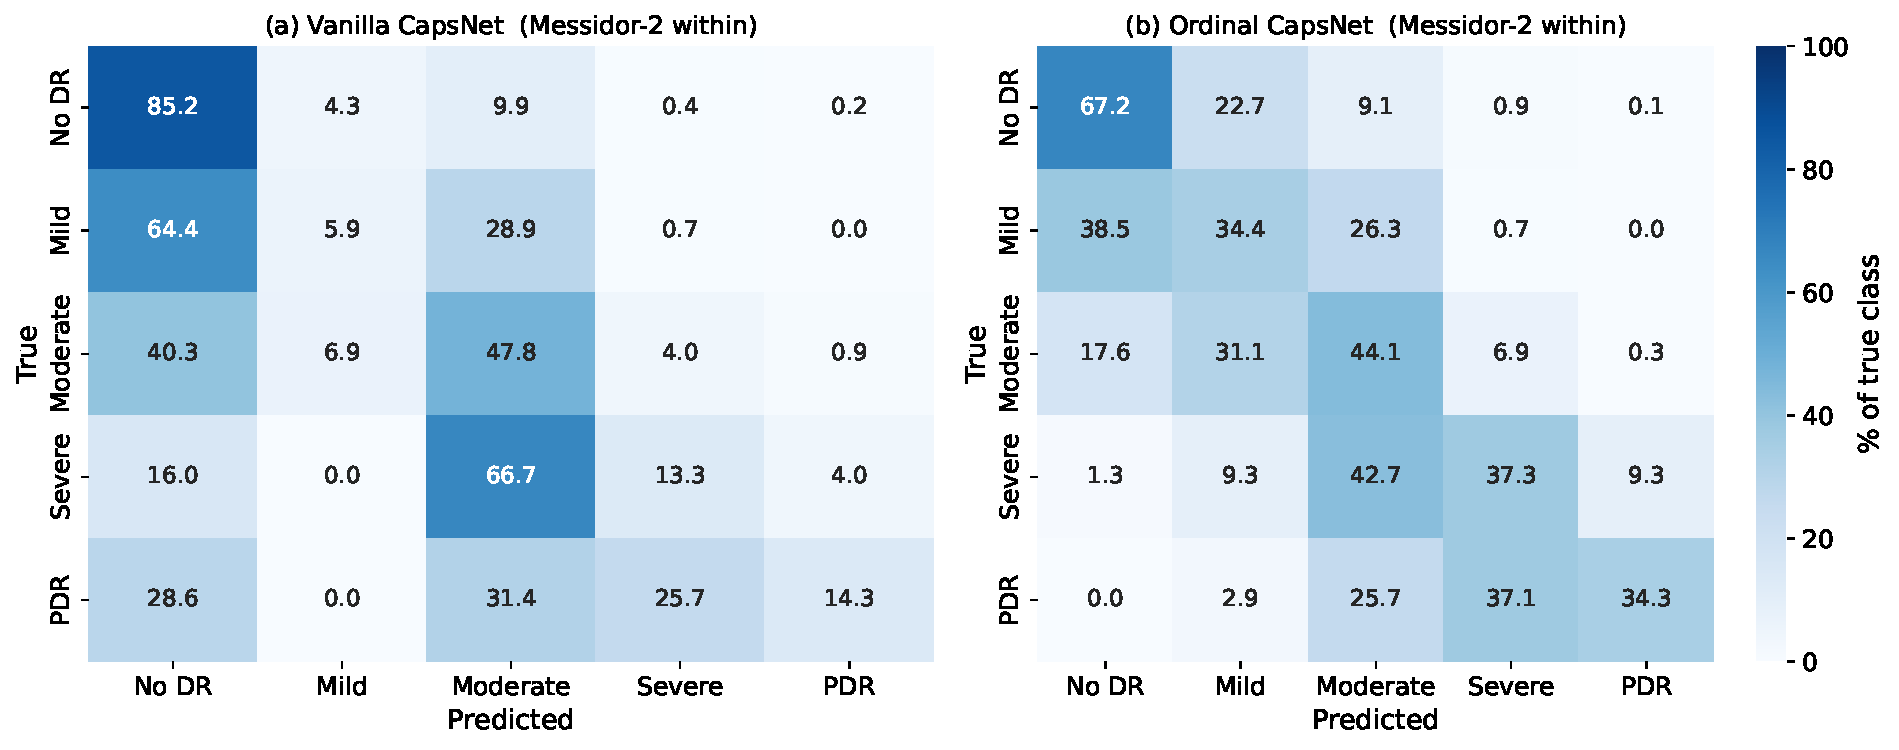
\includegraphics[width=\columnwidth]{figs/fig_g_messidor2_cm_sidebyside.pdf}
    \caption{Messidor-2 confusion matrices (RETFound backbone): Vanilla CapsNet (left) vs Ordinal CapsNet (right), pooled across 5 folds.}
    \label{fig:messidor2_cm}
\end{figure}

\begin{figure}[!t]
    \centering
    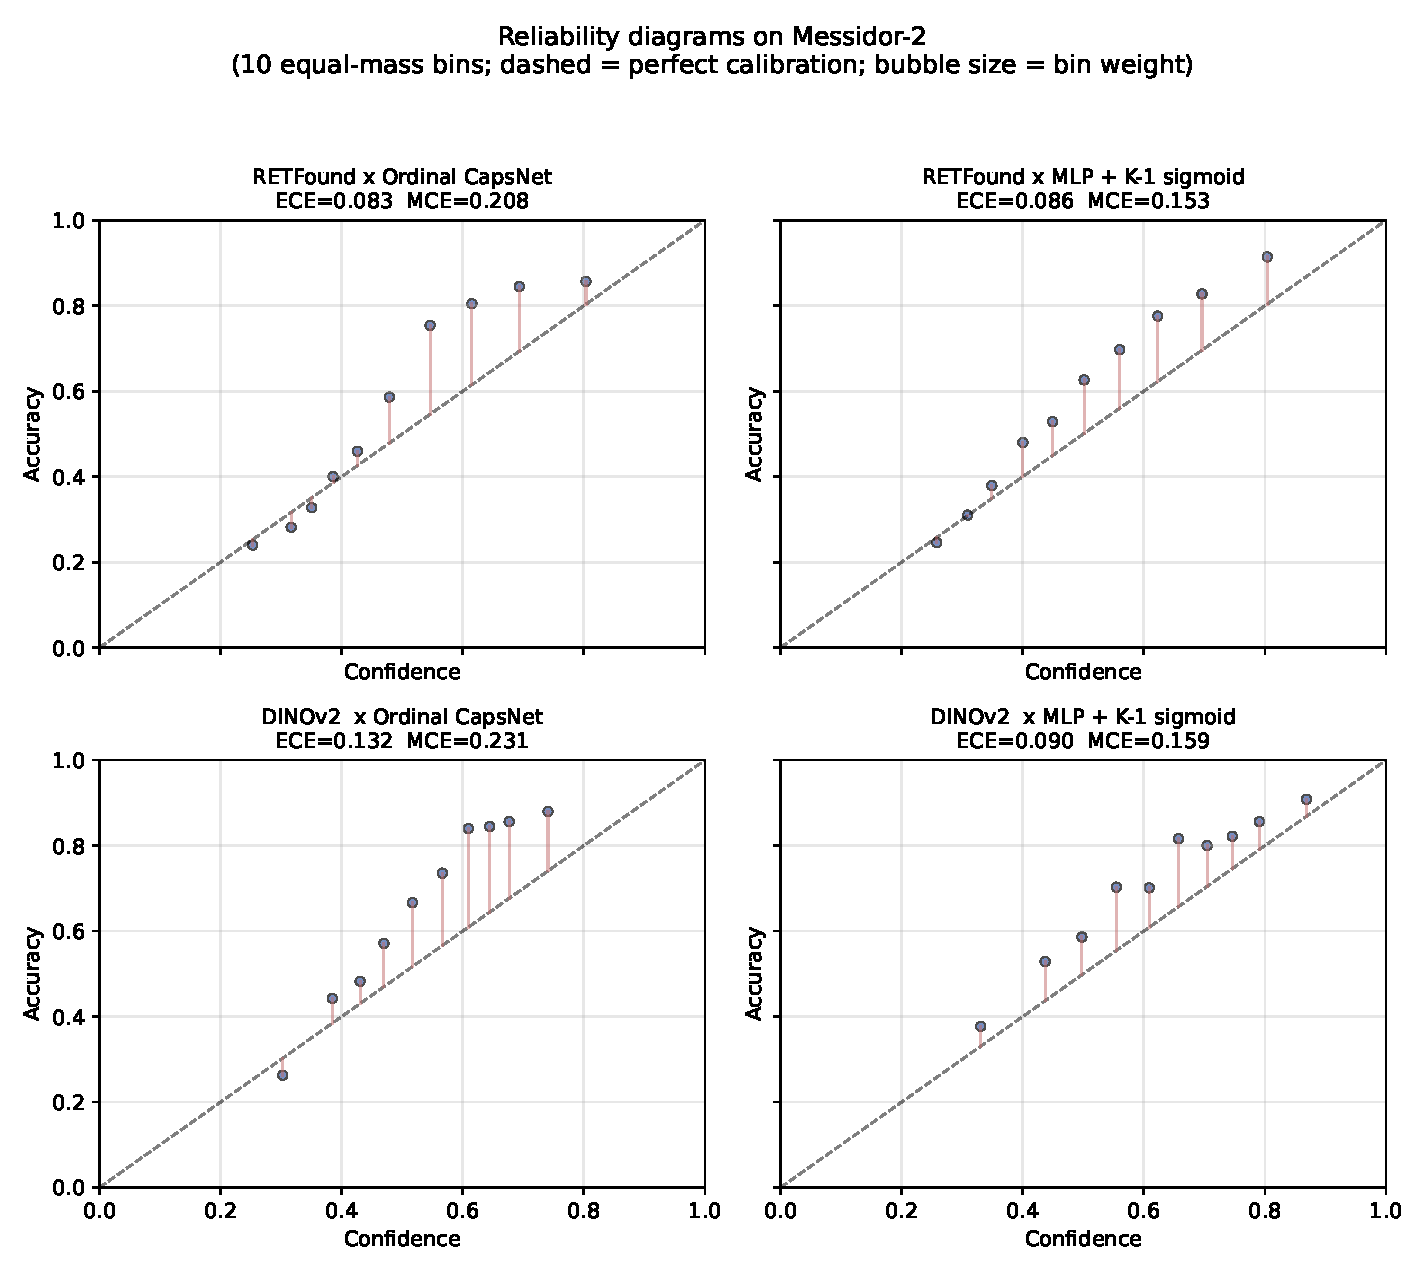
\includegraphics[width=\columnwidth]{figs/fig_reliability_messidor2.pdf}
    \caption{Messidor-2 reliability diagrams for the four head$\times$backbone cells.}
    \label{fig:reliability_messidor2}
\end{figure}

\subsection{Cross-dataset: diagnosis and post-hoc recovery}
\label{sec:cross}

Cross-dataset APTOS$\to$Messidor-2 (no Messidor-2 training) collapses to QWK $\approx 0.01$ across every baseline. Forensics on the pooled 5-fold $\times$ 1,744-sample predictions reveal a near-constant-Grade-0 predictor. Of all samples, $99.4\%$ receive the Grade-0 label under $K{-}1$ thresholding at $0.5$, and $99.9\%$ under argmax of the chain-rule 5-class probabilities. The mean predicted head probabilities are $\bar{P}(y{>}0) = 0.087$, $\bar{P}(y{>}1) = 0.088$, $\bar{P}(y{>}2) = 0.066$, $\bar{P}(y{>}3) = 0.037$. Every head fires below $0.5$ on virtually every sample. This is a feature-distribution shift, not a head failure. The binary AUC stays at $0.61$ (above chance), which means the rank order of predictions is preserved and only the threshold is wrong. Two independent replications confirm this is a property of the frozen RETFound feature space and not of our pipeline. Zoellin et al.\ \cite{ref:zoellin} report frozen-RETFound on Messidor with QKappa exactly $0.0$ (linear-probe adaptation) vs.\ QKappa $0.592$ unfrozen, and frozen-DINOv2 QKappa $0.626$. Poyrazer et al.\ \cite{ref:dinov2_vs_retfound} report a RETFound binary-AUC drop from $0.98$ on APTOS to $0.697$ on external Messidor-2 ($\Delta$AUC $= -0.286$), below even an ImageNet baseline. The frozen-feature cross-dataset collapse from APTOS to Messidor-2 under RETFound-MAE is a stable, reproducible phenomenon in the 2024--2026 literature.

\textbf{Prior-probability shift correction.} For each head, we sort all target-domain samples by severity score $P(y{>}k\,|\,x)$ and assign grades by matching the cumulative distribution to the APTOS \emph{source-domain} prior $\pi$. We call this \emph{rank calibration} throughout. It sits in the prior-shift family opened by Saerens, Latinne and Decaestecker \cite{ref:saerens} but is not their EM estimator, which Table~\ref{tab:uda} evaluates separately and which fails on this transfer; the family has a long follow-up literature (Lipton et al.'s BBSE \cite{ref:bbse}, Alexandari et al.'s MLLS/BCTS \cite{ref:mlls}) that we do not claim novelty against. Our contribution is strictly in applying the source-prior variant as a vulnerability probe for frozen ordinal DR heads. Stronger target-prior estimation (BBSE, MLLS) and full unsupervised domain adaptation (DANN, CORAL, SHOT) are named as future work. The calibration uses no target-domain labels. Table~\ref{tab:cross_messidor2} reports three rows for the ordinal head, namely uncalibrated, APTOS-prior corrected, and oracle (Messidor-2 prior) corrected.

\begin{table*}[!t]
    \caption{APTOS $\to$ Messidor-2 transfer with no target training. Rank calibration uses no target labels; ``Oracle'' uses the true target marginal as an upper bound. The four uncalibrated rows are fold means with across-fold standard deviations; the two calibrated rows are single fold-ensemble predictions, so no deviation is quoted. Read as a vulnerability probe, not a deployment recipe.}
    \label{tab:cross_messidor2}
    \centering
    \footnotesize
    \begin{tabular}{@{}lccc@{}}
        \toprule
        Method                                                         & QWK                 & Bin.\ Sens.\      & Bin.\ AUC        \\
        \midrule
        MLP + CE                                                       & $0.0024 \pm 0.0008$ & ---               & $0.585$           \\
        MLP + MSE                                                      & $0.0076 \pm 0.0039$ & ---               & $0.566$           \\
        Vanilla CapsNet                                                & $0.0035 \pm 0.0034$ & ---               & $0.570$           \\
        Ordinal CapsNet (uncalibrated)                                 & $0.0301 \pm 0.0185$ & $2.0\%$           & $\mathbf{0.620}$  \\
        \textbf{Ordinal CapsNet + rank calib.\ (APTOS prior, no labels)} & $\mathbf{0.2399}$   & $\mathbf{53.8\%}$ & $0.632$           \\
        Ordinal CapsNet + rank calib.\ (oracle prior, upper bound) & $0.2783$            & ---               & ---               \\
        \bottomrule
    \end{tabular}
\end{table*}

Source-prior rank calibration lifts the ordinal ranking signal from QWK $0.030$ to $0.240$ and the binary sensitivity from $2.0\%$ to $53.8\%$ at an essentially unchanged AUC of $0.632$. The AUC is almost identical in all three rows, confirming that the rank information is preserved and the intervention is purely a threshold fix. We emphasise that QWK $0.240$ remains in the Landis-Koch \emph{fair} band ($0.21$ to $0.40$) and is far below the $\approx$0.60 clinical-agreement threshold. A binary sensitivity of $53.8\%$ would miss nearly half of all referable patients. The intervention is therefore a \emph{diagnostic probe} demonstrating that the cross-dataset collapse is mechanistically a threshold miscalibration rather than a feature-space destruction, not a clinical-deployment recipe. Fig.~\ref{fig:messidor2_roc} shows the binary-referable ROC.

\begin{figure}[!t]
    \centering
    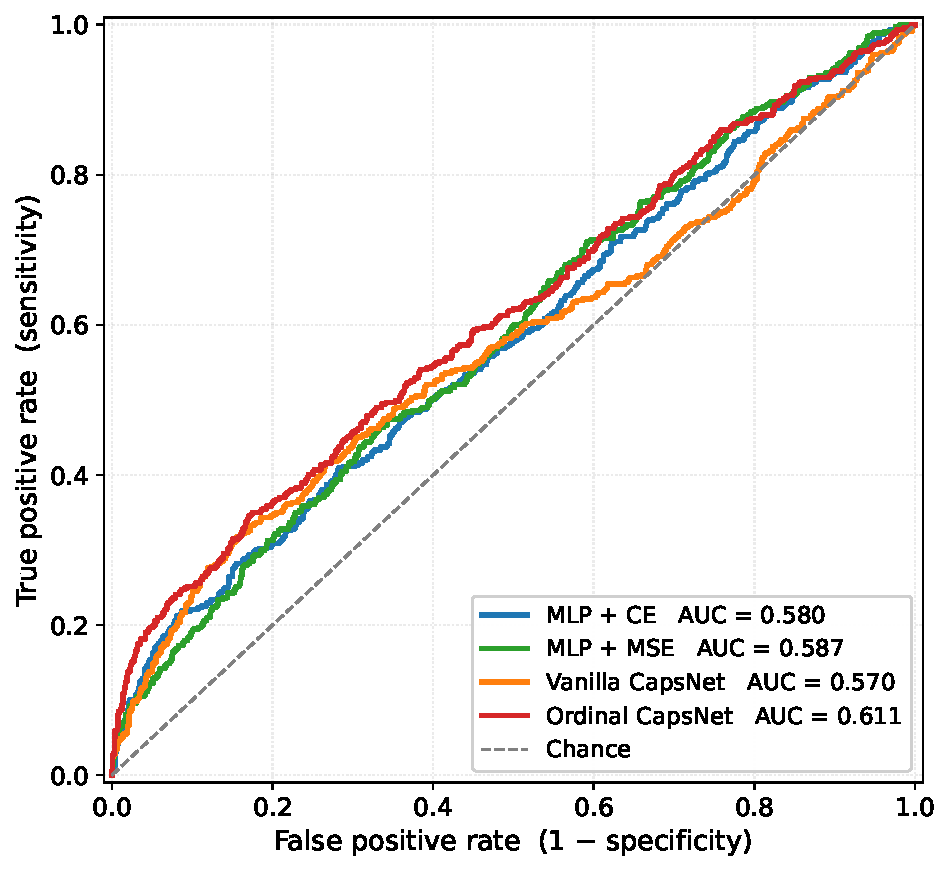
\includegraphics[width=\columnwidth]{figs/fig_h_messidor2_roc.pdf}
    \caption{APTOS $\to$ Messidor-2 binary-referable ROC (grade $\geq 2$). The ordinal head's AUC of $0.625$ is well above chance, which is why post-hoc rank calibration can recover such a large fraction of the QWK loss. The rank order is intact and only the threshold is wrong.}
    \label{fig:messidor2_roc}
\end{figure}

The takeaway is methodological, not operational. Under frozen RETFound-MAE features, the APTOS $\to$ Messidor-2 transfer failure is driven primarily by a $K{-}1$-threshold miscalibration, namely the $\bar{P}(y{>}0)$ distributional shift from $0.51$ to $0.087$. A source-prior intervention exposes this structure clearly but does not cross the clinical threshold. Genuine cross-dataset deployment requires either a stronger backbone (our within-Messidor-2 DINOv2 $\times$ MLP-K1 already reaches QWK $0.76$, see Section~\ref{sec:messidor-within}), label-shift estimation on the target domain \cite{ref:bbse,ref:mlls}, or full unsupervised domain adaptation. We concur with Ahamed et al.\ \cite{ref:dr_conformal}, who observe that data-augmentation choices interact non-trivially with conformal coverage on DR grading; a similar data-level intervention on the source side is a natural complement to the head-level probe reported here.

\subsection{IDRiD}
On IDRiD with RETFound features, the Ordinal CapsNet reaches validation QWK $0.7595$ but only $0.4232 \pm 0.019$ on the 103-image official test. Every baseline drops by $0.29$ to $0.35$ QWK from validation to test, indicating a dataset-wide distribution shift between the 413-image train set and the held-out test. APTOS $\to$ IDRiD transfer reaches QWK $0.2788$. Section~\ref{sec:idrid-dinov2} repeats all of this under DINOv2, where both numbers improve substantially and the val$\to$test gap narrows.

\subsection{Training dynamics and compute}
\label{sec:compute}
Each frozen 5-fold run completes in roughly 115 seconds on an Apple M-series MacBook (MPS backend). The LoRA 5-fold run takes $\approx$65--85 min/fold, or $\approx$16h for 3 seeds $\times$ 5 folds on the same laptop. DINOv2 feature extraction for both datasets took roughly 7 minutes on MPS.



\subsection{Backbone $\times$ tuning: completing the matrix}
\label{sec:backbone-tuning}
\begin{table}[!t]
\centering
\caption{Backbone $\times$ tuning interaction on APTOS (Ordinal CapsNet head, 3 seeds $\times$ 5-fold CV). LoRA is rank 8 on \texttt{attn.qkv} in every block.}
\label{tab:backbonetuning}
\begin{tabular}{lccc}
\toprule
Backbone & Frozen & $+$ LoRA & $\Delta$ tuning \\
\midrule
RETFound ViT-L/16 & $0.8923 \pm 0.0002$ & $0.9143 \pm 0.0006$ & $+0.0220$ \\
DINOv2 ViT-L/14   & $0.9074 \pm 0.0029$ & $0.9156 \pm 0.0013$ & $+0.0081$ \\
\midrule
$\Delta$ backbone & $+0.0152$ & $+0.0013$ & \\
\bottomrule
\end{tabular}
\end{table}

The submitted paper reported three of these four cells; the DINOv2 $+$ LoRA cell was omitted for compute reasons, which reviewers correctly identified as leaving the comparison incomplete. Filling it changes the reading of our own headline result.

Frozen, the backbone gap is $+0.0152$ QWK in DINOv2's favour, which is the basis for the claim that the backbone is the dominant lever. Under LoRA that gap shrinks to $+0.0013$ --- essentially nothing. The reason is an interaction rather than a ceiling: LoRA is worth $+0.0220$ on RETFound but only $+0.0081$ on DINOv2, so rank-8 adaptation recovers most of what the weaker backbone was missing. Best overall is DINOv2 $+$ LoRA at $0.9156$ QWK (accuracy $0.8300$, MAE $0.204$), but it beats RETFound $+$ LoRA by a margin comparable to the across-seed spread.

The refined statement is therefore this: the backbone dominates \emph{when features are frozen}, and that is the regime the efficiency argument of this paper targets. Once even a small number of adapter parameters is trainable, backbone choice becomes close to irrelevant on APTOS, and $1.08$M adapter parameters substitute for the difference between a domain-specific and a generalist ViT-L. For a practitioner the decision rule is not ``pick the better backbone'' but ``if you can afford any fine-tuning at all, backbone choice stops mattering; if you cannot, it matters a great deal''.


\subsection{Does the adapter substitution hold on a second dataset?}
\label{sec:messidor-lora}
The fine-tuning tiers above are measured on APTOS alone, which makes every
conclusion about adapters single-dataset. We therefore repeated the LoRA tier
on Messidor-2 under an identical protocol (rank 8 on \texttt{attn.qkv}, same
optimiser and learning rates, stratified 5-fold CV on the $1{,}744$ gradable
images).

LoRA lifts Messidor-2 from QWK $0.6021$ frozen to $0.7097$, a gain of $+0.1076$ --- roughly
five times the $+0.0220$ it buys on APTOS --- and it cuts fold-to-fold variance
threefold ($0.0152$ against $0.0454$), so the adapted model is markedly more
stable on the harder cohort.

The gain does not, however, close the backbone gap. Frozen DINOv2 reaches
$0.7586$ on the same split, so RETFound with adapters remains $0.0488$ behind a
better backbone used with no training at all. This qualifies the APTOS
reading of Section~\ref{sec:backbone-tuning}, where LoRA erased a $+0.0151$
backbone gap entirely. Adapters substitute for backbone quality when the gap
is small; when the domain shift is large they recover roughly two-thirds of
it ($+0.1076$ of $0.1565$) and no more. Stated as a single rule: parameter-
efficient adaptation narrows backbone differences but does not reliably
eliminate them, and the residual grows with the difficulty of the target
domain.

\subsection{Rank-monotonicity: projection versus repair}
\label{sec:monotone-results}
\begin{table}[!t]
\centering
\caption{Effect of the rank-monotonicity projection of Eq.~\eqref{eq:monotone}. A is the submitted decode (product, clipped, renormalised); C is the projection with exact cumulative differences. ``Viol.'' is the continuous-head violation rate. Metrics here use $\arg\max_k P(y{=}k)$ of the decoded distribution, so column A differs slightly from the ECE in Table~\ref{tab:calibration}, which scores the Eq.~\eqref{eq:predict} threshold rule.}
\label{tab:monotone}
\begin{tabular}{llccc}
\toprule
Dataset & Model & Viol. & ECE (A) & ECE (C) \\
\midrule
APTOS & RETFound $\times$ Ordinal CapsNet & 55.6\% & 0.1469 & $\mathbf{0.0715}$ \\
 & RETFound $\times$ MLP + K-1 sigmoid & 46.2\% & 0.1026 & $\mathbf{0.0552}$ \\
 & DINOv2 $\times$ Ordinal CapsNet & 56.7\% & 0.1238 & $\mathbf{0.0580}$ \\
 & DINOv2 $\times$ MLP + K-1 sigmoid & 44.5\% & 0.1060 & $\mathbf{0.0562}$ \\
 & RETFound $\times$ Ordinal CapsNet + LoRA & 56.2\% & 0.1339 & $\mathbf{0.0549}$ \\
\midrule
Messidor-2 & RETFound $\times$ Ordinal CapsNet & 37.8\% & 0.1054 & $\mathbf{0.0459}$ \\
 & RETFound $\times$ MLP + K-1 sigmoid & 4.2\% & 0.0860 & $\mathbf{0.0387}$ \\
 & DINOv2 $\times$ Ordinal CapsNet & 62.2\% & 0.1207 & $\mathbf{0.0580}$ \\
 & DINOv2 $\times$ MLP + K-1 sigmoid & 48.5\% & 0.0835 & $\mathbf{0.0329}$ \\
\bottomrule
\end{tabular}
\end{table}

The continuous heads violate rank-monotonicity on $4.2$ to $62.2\%$ of samples depending on the configuration, two orders of magnitude more often than the $0.3\%$ reported by the thresholded consistency count, which only registers contradictions among the hard $\hat{p}_k > 0.5$ decisions. Replacing clip-and-renormalise with the projection of Eq.~\eqref{eq:monotone} roughly halves ECE on every one of the nine cells (mean reduction $53\%$), for a QWK cost of $0.004$ to $0.014$. Unlike temperature scaling this requires no held-out split and no fitted parameter. The capsule heads violate monotonicity substantially more often than the MLP-K1 baseline at matched backbone ($55.6\%$ vs.\ $46.2\%$ on APTOS/RETFound, $37.8\%$ vs.\ $4.2\%$ on Messidor-2/RETFound), which is the same ordering we observe in ECE and, below, in set contiguity.

\subsection{Ordinal contiguous prediction sets}
\label{sec:ocp-results}
\begin{table*}[!t]
\centering
\caption{OCP versus label-set scores at $\alpha = 0.10$, over five calibration/test splits. The first three columns give the fraction of sets that skip an intermediate grade; OCP is zero by construction.}
\label{tab:ocp}
\begin{tabular}{llccc cc cc}
\toprule
& & \multicolumn{3}{c}{Non-contiguous rate} & \multicolumn{2}{c}{APS} & \multicolumn{2}{c}{OCP (ours)} \\
\cmidrule(lr){3-5} \cmidrule(lr){6-7} \cmidrule(lr){8-9}
Dataset & Model & LAC & APS & RAPS & cov. & $|S|$ & cov. & $|S|$ \\
\midrule
APTOS & RETFound $\times$ Ordinal CapsNet & 5.1\% & 12.2\% & 12.6\% & 0.943 & 1.81 & 0.943 & 1.88 \\
 & RETFound $\times$ MLP + K-1 sigmoid & 2.3\% & 8.4\% & 8.7\% & 0.939 & 1.87 & 0.938 & 1.91 \\
 & DINOv2 $\times$ Ordinal CapsNet & 2.3\% & 8.1\% & 8.3\% & 0.948 & 1.76 & 0.948 & 1.81 \\
 & DINOv2 $\times$ MLP + K-1 sigmoid & 1.8\% & 7.3\% & 7.7\% & 0.945 & 1.80 & 0.946 & 1.84 \\
 & RETFound $\times$ Ordinal CapsNet + LoRA & 0.7\% & 4.9\% & 5.0\% & 0.942 & 1.69 & 0.943 & 1.71 \\
\midrule
Messidor-2 & RETFound $\times$ Ordinal CapsNet & 5.9\% & 12.8\% & 12.9\% & 0.903 & 2.50 & 0.901 & 2.54 \\
 & RETFound $\times$ MLP + K-1 sigmoid & 0.9\% & 3.8\% & 3.8\% & 0.902 & 2.48 & 0.906 & 2.51 \\
 & DINOv2 $\times$ Ordinal CapsNet & 4.1\% & 9.9\% & 10.2\% & 0.895 & 2.03 & 0.892 & 2.03 \\
 & DINOv2 $\times$ MLP + K-1 sigmoid & 0.6\% & 3.7\% & 3.6\% & 0.904 & 2.03 & 0.903 & 2.02 \\
\bottomrule
\end{tabular}
\end{table*}

Between $0.6$ and $5.9\%$ of LAC sets and $3.7$ to $12.8\%$ of APS sets are non-contiguous, so a per-configuration measurement is necessary: no single rate characterises the grid. OCP removes all of them while matching APS coverage, at a mean set-size cost of $+0.04$ grades (worst case $+0.066$); on Messidor-2 with DINOv2 $\times$ MLP-K1 it is $0.015$ \emph{smaller} than APS. Ordinal coherence is therefore effectively free, and the capsule heads again pay the larger incoherence penalty ($12.8\%$ vs.\ $3.8\%$ on Messidor-2/RETFound).

\subsection{Fine-tuning tiers}
\label{sec:finetune-results}
\begin{table}[!t]
\centering
\caption{Fine-tuning tiers on APTOS, 5-fold CV on identical splits; tiers differ only in which backbone parameters receive gradients. $n$ is the number of model seeds; the uncertainty is the across-seed standard deviation.}
\label{tab:finetune}
\begin{tabular}{llccccc}
\toprule
Tier & Trainable & QWK & Acc & MAE & $n$ \\
\midrule
\multicolumn{6}{l}{\emph{RETFound ViT-L/16}} \\
\quad Frozen head only & 295{,}168 & $0.8923 \pm 0.0002$ & 0.7935 & --- & 3 \\
\quad LoRA $r{=}8$ & 1{,}081{,}600 & $0.9143 \pm 0.0006$ & 0.8240 & 0.212 & 3 \\
\quad Progressive (last 4) & 50{,}813{,}184 & $0.9169 \pm 0.0015$ & 0.8290 & 0.203 & 3 \\
\quad Full fine-tune & 304{,}383{,}232 & $0.8801 \pm 0.0105$ & 0.7953 & 0.262 & 3 \\
\midrule
\multicolumn{6}{l}{\emph{DINOv2 ViT-L/14}} \\
\quad Frozen head only & 295{,}168 & $0.9074 \pm 0.0029$ & 0.8037 & --- & 3 \\
\quad LoRA $r{=}8$ & 1{,}081{,}600 & $0.9156 \pm 0.0013$ & 0.8300 & 0.204 & 3 \\
\quad Progressive (last 4) & 50{,}813{,}184 & $0.9114 \pm 0.0000$ & 0.8179 & 0.217 & 1 \\
\quad Full fine-tune & 304{,}368{,}640 & $0.5383 \pm 0.0000$ & 0.5590 & 0.701 & 1 \\
\bottomrule
\end{tabular}
\end{table}

Full fine-tuning is \emph{worse} than training no backbone parameter at all, on both backbones. On RETFound it reaches $0.8801$ against $0.8923$ frozen, despite $1{,}031\times$ more trainable weights, and MAE degrades in step ($0.262$ against $0.212$). Its across-seed spread is also $46$ times the frozen tier's ($0.0105$ against $0.0002$), so the failure is erratic rather than a uniform shift.

On DINOv2 the same recipe fails outright. Mean QWK is $0.5383$, and the run is unstable rather than merely poor: one of the five folds collapsed to a constant predictor (QWK exactly $0$, validation accuracy pinned at the majority-class rate), and excluding that fold the remaining four average only $0.673$ against $0.907$ frozen. We attribute this to the learning rate rather than to the backbone: all tiers share the $10^{-4}$ backbone learning rate chosen for LoRA, which is far too aggressive when every one of $304$M parameters is updated on $2{,}636$ images. We did not tune it per tier, and a properly annealed schedule would very likely recover much of the loss. The defensible claim is therefore about the recipe, not about DINOv2: full fine-tuning at a parameter-efficient tier's hyperparameters is not merely wasteful but actively unstable.

Between the two useful tiers, progressive unfreezing of the last four blocks and LoRA are statistically indistinguishable on RETFound ($+0.0026$ with across-seed standard deviations of $0.0015$ and $0.0006$), and LoRA is ahead on DINOv2 ($0.9156$ against $0.9114$). LoRA therefore matches the best tier with $47\times$ fewer trainable parameters. The parameter-efficiency curve is non-monotonic on both backbones, peaking far below full capacity.

\subsection{Is the miscalibration the loss or the architecture?}
\label{sec:loss-factorial}
\begin{table}[!t]
\centering
\caption{Loss $\times$ head factorial on APTOS, 3 seeds $\times$ 5-fold CV, everything else held fixed. ECE is reported under the submitted product decode and under the projection of Eq.~\eqref{eq:monotone}.}
\label{tab:lossfactorial}
\begin{tabular}{llccccc}
\toprule
Head & Loss & QWK & Acc & ECE (prod.) & ECE (proj.) & Viol. \\
\midrule
Ordinal CapsNet & margin & $0.8922 \pm 0.0013$ & 0.7904 & 0.1581 & 0.0811 & 58.3\% \\
 & BCE & $0.8867 \pm 0.0006$ & 0.7853 & 0.0791 & 0.0323 & 50.3\% \\
 & focal & $0.8908 \pm 0.0011$ & 0.7943 & 0.2091 & 0.1122 & 46.9\% \\
\midrule
MLP + $K{-}1$ & margin & $0.8847 \pm 0.0008$ & 0.7929 & 0.1050 & 0.0555 & 50.9\% \\
 & BCE & $0.8856 \pm 0.0016$ & 0.7897 & 0.0181 & 0.0221 & 28.4\% \\
 & focal & $0.8846 \pm 0.0011$ & 0.7896 & 0.1771 & 0.0904 & 19.3\% \\
\bottomrule
\end{tabular}
\end{table}

The submitted paper attributed the capsule head's poor calibration to the Sabour margin loss, but never varied the two factors independently: every capsule row used the margin loss, so loss and architecture were confounded. Running the full factorial separates them, and both turn out to matter, by comparable amounts.

The loss main effect is the larger of the two. Replacing the margin loss with plain binary cross-entropy on the same heads improves ECE by $-0.0790$ for the capsule head and $-0.0869$ for the MLP head. Focal loss is worse than either. The architecture main effect is present under every loss and does not wash out: at matched loss the capsule head is worse calibrated by $+0.0532$ (margin), $+0.0610$ (BCE) and $+0.0320$ (focal). So the original attribution was half right. The margin loss is genuinely miscalibrating, but a capsule head trained with a proper scoring rule is still worse calibrated than an MLP trained the same way.

The practically useful cell is MLP+$K{-}1$ with BCE, at ECE $0.0181$ against $0.1581$ for the submitted capsule-plus-margin configuration --- better calibrated by a factor of $8.7$ --- for a QWK cost of $-0.0065$. Two further observations. Rank-monotonicity violations track the same ordering ($28.4\%$ for MLP+BCE against $58.3\%$ for capsule+margin), reinforcing that these are three views of one underlying property. And the projection of Eq.~\eqref{eq:monotone} helps every configuration except the best-calibrated one, where it is marginally harmful ($0.0221$ against $0.0181$): once the decoded probabilities are already close to calibrated, enforcing monotonicity has nothing left to repair.

\subsection{Input resolution}
\label{sec:resolution}
\begin{table}[!t]
\centering
\caption{Input resolution on APTOS with frozen RETFound features, 3 seeds $\times$ 5-fold CV. The $448$ rows resample the pretrained position embedding onto a $28{\times}28$ grid.}
\label{tab:resolution}
\begin{tabular}{llccc}
\toprule
Head & Res. & QWK & Acc & Macro-F1 \\
\midrule
Ordinal CapsNet & $224$ & $0.8923 \pm 0.0002$ & 0.7935 & 0.6259 \\
Ordinal CapsNet & $448$ & $0.8828 \pm 0.0008$ & 0.7785 & 0.6036 \\
\midrule
MLP + $K{-}1$ & $224$ & $0.8849 \pm 0.0015$ & 0.7976 & 0.6235 \\
MLP + $K{-}1$ & $448$ & $0.8771 \pm 0.0011$ & 0.7832 & 0.6106 \\
\bottomrule
\end{tabular}
\end{table}

A reasonable objection to the $224$ crop is that downsampling a multi-megapixel fundus photograph by roughly an order of magnitude in each dimension may destroy the small, sparse lesions -- microaneurysms in particular -- that separate the lower grades. We tested it directly. Features were re-extracted at $448{\times}448$ from a losslessly cached $512$-pixel copy of each image, using the identical transform scaled to the new size, with the pretrained absolute position embedding resampled bicubically from $14{\times}14$ to $28{\times}28$ patches. Everything downstream is unchanged.

Quadrupling the pixel count makes grading \emph{worse}, by $-0.0094$ QWK for the capsule head and $-0.0079$ for the MLP head. The effect is consistent across all three seeds and far outside seed noise (across-seed standard deviations $\leq 0.0015$ throughout), and it appears with both heads, so it is a property of the backbone rather than of the ordinal head. The likely mechanism is that RETFound was pretrained at $224$: running it at $448$ forces its learned position embedding onto a token grid it never saw, and that distribution mismatch costs more than the recovered lesion detail gains. The practical reading is not that fine detail is irrelevant to DR grading, but that it cannot be recovered by feeding a $224$-pretrained ViT larger inputs; a backbone pretrained at the target resolution would be needed to test the lesion-detail hypothesis properly.




\subsection{Computational complexity}
\label{sec:compute}
\begin{table}[!t]
\centering
\caption{Complexity on one NVIDIA A100-SXM4-40GB. Forward FLOPs are traced per image with \texttt{torch.utils.flop\_counter} (exact op counts, not analytic estimates). Peak memory and throughput are measured at the largest batch that fits; throughput is a training step for trainable rows and a no-grad forward for the frozen backbones.}
\label{tab:compute}
\begin{tabular}{lcccc}
\toprule
Component & Trainable & FLOPs/img & Peak (MiB) & img/s \\
\midrule
Ordinal CapsNet head & 295{,}168 & 0.59\,MFLOP & 32 & 9{,}589 \\
MLP + $K{-}1$ head & 329{,}220 & 0.66\,MFLOP & 26 & 28{,}536 \\
RETFound ViT-L/16 (frozen) & 0 & 123.1\,GFLOP & 1{,}849 & 144 \\
DINOv2 ViT-L/14 (frozen) & 0 & 162.0\,GFLOP & 1{,}963 & 107 \\
RETFound $+$ LoRA $r{=}8$ & 1{,}081{,}600 & 123.4\,GFLOP & 15{,}019 & 65 \\
RETFound full fine-tune & 304{,}383{,}232 & 123.4\,GFLOP & 25{,}293 & 45 \\
\bottomrule
\end{tabular}
\end{table}

Reviewers noted that the submitted paper timed everything on a consumer laptop and asked for FLOPs, peak GPU memory and throughput on a server GPU. Three things follow from the measurement.

First, the head choice is computationally irrelevant. The backbone costs about 208{,}722 times the FLOPs of the head it feeds ($123.1$\,GFLOP against $0.59$\,MFLOP per image), so the capsule-versus-MLP debate that occupies much of this paper is, in compute terms, noise on top of the backbone decision. The ``backbone dominates the head'' finding holds on compute as well as on QWK, by five orders of magnitude.

Second, capsule routing is $3.0$ times \emph{slower} to train than the MLP head despite having fewer parameters and fewer FLOPs ($9{,}589$ against $28{,}536$ images/s). Three sequential routing iterations serialise into many small kernel launches that the GPU cannot amortise --- a real cost that a parameter count hides entirely.

Third, DINOv2's accuracy advantage is not free: patch-14 tokenisation yields 257 tokens against RETFound's 197, costing $162.0$\,GFLOP against $123.1$\,GFLOP per image and running $26$\% slower. LoRA against full fine-tuning is $281$ times fewer trainable parameters, $1.68$ times less peak memory ($14.7$ against $24.7$\,GiB) and $1.46$ times the throughput.

A caveat that matters for the efficiency claim. The frozen tier does not benefit from a server GPU at all: at $\sim\!10^5$ parameters over 1024-dimensional vectors the step is bound by Python and kernel-launch latency rather than arithmetic, and a full 5-fold frozen run takes $363$\,s on the A100 against $385$\,s on CPU and $\approx\!115$\,s on the M-series laptop used for the original experiments. The laptop is the fastest of the three. The A100 matters only for the LoRA and fine-tuning tiers.

\subsection{Domain adaptation for APTOS $\to$ Messidor-2}
\label{sec:uda}
\begin{table}[!t]
\centering
\caption{Label-free adaptation for APTOS $\to$ Messidor-2, Ordinal CapsNet on frozen RETFound features, 5 folds. Feature alignment maps the target into the source space; label correction reweights or reassigns the decoded posterior. Only the two oracle rows use target labels.}
\label{tab:uda}
\begin{tabular}{llccc}
\toprule
Align & Label correction & QWK & rDR sens. & rDR spec. \\
\midrule
--- & --- & $0.0132 \pm 0.0090$ & 0.005 & 1.000 \\
z-score & --- & $0.1420 \pm 0.0165$ & 0.502 & 0.633 \\
CORAL & --- & $0.1742 \pm 0.0211$ & 0.467 & 0.687 \\
--- & BBSE & $0.0494 \pm 0.0236$ & 0.179 & 0.858 \\
--- & EM & $0.0005 \pm 0.0010$ & 0.000 & 1.000 \\
CORAL & EM & $0.1399 \pm 0.0384$ & 0.496 & 0.653 \\
--- & rank calib. & $0.2266 \pm 0.0354$ & 0.531 & 0.638 \\
CORAL & rank calib. & $0.1860 \pm 0.0105$ & 0.523 & 0.636 \\
--- & oracle prior & $0.0015 \pm 0.0013$ & 0.001 & 1.000 \\
--- & rank calib. (oracle prior) & $0.2619 \pm 0.0414$ & 0.384 & 0.781 \\
\bottomrule
\end{tabular}
\end{table}

Reviewers asked whether standard unsupervised domain adaptation would rescue this transfer, given that our post-hoc correction leaves it below clinical usefulness. We tested the adaptations that apply when the backbone is frozen and features are cached, factorised into the two shifts involved: second-order feature alignment (CORAL, in the correlation-alignment sense of Sun and Saenko \cite{ref:coral_da}, not the ordinal-regression method of the same acronym) and per-domain standardisation for covariate shift; and BBSE \cite{ref:bbse}, EM \cite{ref:saerens} and our rank calibration for label shift.

No adaptation beats what the paper already does. Feature alignment is a real effect --- CORAL alone lifts QWK from $0.0132$ to $0.1742$, a factor of $13$ --- but it remains below rank calibration at $0.2266$, and stacking the two is worse than either ($0.1860$). The $0.2266$ here is the fold mean, against the $0.2399$ fold-ensemble figure of Table~\ref{tab:cross_messidor2}; every row of this table is a fold mean so that the comparison is like-for-like. Every row stays far below the $\approx 0.60$ clinical-agreement threshold, so the conclusion is unchanged; it is now supported rather than asserted.

The instructive failure is posterior reweighting. EM and BBSE on unaligned features score $0.0005$ and $0.0494$, no better than doing nothing, and even supplying the \emph{true} target prior reaches only $0.0015$. The decoded posterior has saturated at $P(y{=}0) \approx 1$, so multiplicative reweighting cannot move the arg-max however extreme the ratio. Rank calibration works precisely because it uses only the ordering and reassigns labels outright. This is the mechanistic reason our correction is the right tool for this failure mode, and why the reviewers' suggested alternatives underperform it here.

\subsection{IDRiD under both backbones}
\label{sec:idrid-dinov2}
\begin{table}[!t]
\centering
\caption{IDRiD, 5-fold CV on the 413 training images evaluated on the official 103-image test set. Validation QWK is the in-fold mean.}
\label{tab:idrid_backbone}
\begin{tabular}{lccccc}
\toprule
& \multicolumn{2}{c}{RETFound} & \multicolumn{2}{c}{DINOv2} & \\
\cmidrule(lr){2-3}\cmidrule(lr){4-5}
Model & val & test & val & test & $\Delta$ test \\
\midrule
MLP + CE & 0.7575 & $0.4078 \pm 0.0584$ & 0.8715 & $0.6276 \pm 0.0348$ & $+0.2199$ \\
MLP + MSE & 0.7551 & $0.4614 \pm 0.0289$ & 0.8694 & $0.6573 \pm 0.0205$ & $+0.1959$ \\
Vanilla CapsNet & 0.7484 & $0.4124 \pm 0.0583$ & 0.8671 & $0.6183 \pm 0.0471$ & $+0.2059$ \\
Ordinal CapsNet & 0.7595 & $0.4232 \pm 0.0192$ & 0.8706 & $0.6393 \pm 0.0271$ & $+0.2160$ \\
\bottomrule
\end{tabular}
\end{table}

The submitted paper reported IDRiD under RETFound only, and drew two conclusions from it: that every model loses roughly $0.30$ QWK from validation to the official test split, and that this is a property of the IDRiD split rather than of any one head. Both survive, but the second needs qualifying, because the size of the drop is strongly backbone-dependent.

Swapping in DINOv2 lifts test QWK by $+0.196$ to $+0.220$ on every one of the four models, moving the best from $0.4614$ to $0.6573$. The validation-to-test gap narrows from $0.29$ to $0.35$ to $0.21$ to $0.25$, so the ``IDRiD split is simply hard'' reading is only partly right: roughly a third of the gap was attributable to the backbone rather than to the split.

The cross-dataset result changes more sharply still. APTOS$\to$IDRiD transfer with no IDRiD training rises from QWK $0.2788$ under RETFound to $0.6259$ under DINOv2. That is within noise of the $0.6573$ obtained by training on IDRiD directly, and it sits at the boundary of the $\approx 0.60$ clinical-agreement threshold that the APTOS$\to$Messidor-2 transfer never approaches. The pessimistic cross-dataset conclusion of the submitted paper is therefore specific to RETFound-MAE features rather than a general statement about frozen-feature transfer, and we have restated it accordingly. Messidor-2 remains the harder target: its transfer failure is a threshold collapse (Section~\ref{sec:cross}) that a stronger backbone alone does not fix.

\subsection{Clinical screening performance}
\label{sec:clinical}
\begin{table}[!t]
\centering
\caption{Referable-DR screening (grade $\geq 2$), read off the head output $P(y{>}1)$ at threshold $0.5$. NHS marks whether the row clears the screening bar (sensitivity $\geq 0.85$, specificity $\geq 0.80$).}
\label{tab:clinical}
\begin{tabular}{llccccc}
\toprule
Dataset & Model & AUROC & Sens. & Spec. & Bal.\ acc & NHS \\
\midrule
APTOS & RETFound $\times$ Ordinal CapsNet & 0.976 & 0.948 & 0.909 & 0.928 & pass \\
 & RETFound $\times$ MLP + K-1 sigmoid & 0.977 & 0.939 & 0.913 & 0.926 & pass \\
 & DINOv2 $\times$ Ordinal CapsNet & 0.978 & 0.957 & 0.914 & 0.936 & pass \\
 & DINOv2 $\times$ MLP + K-1 sigmoid & 0.981 & 0.954 & 0.916 & 0.935 & pass \\
 & RETFound $\times$ Ordinal CapsNet + LoRA & 0.981 & 0.954 & 0.931 & 0.942 & pass \\
\midrule
Messidor-2 & RETFound $\times$ Ordinal CapsNet & 0.820 & 0.639 & 0.853 & 0.746 & fail \\
 & RETFound $\times$ MLP + K-1 sigmoid & 0.825 & 0.619 & 0.852 & 0.735 & fail \\
 & DINOv2 $\times$ Ordinal CapsNet & 0.893 & 0.720 & 0.949 & 0.835 & fail \\
 & DINOv2 $\times$ MLP + K-1 sigmoid & 0.915 & 0.744 & 0.928 & 0.836 & fail \\
\bottomrule
\end{tabular}
\end{table}


Because head $k$ emits $P(y{>}k)$ directly, the referable-DR detector requires no additional thresholding or class marginalisation; it is simply head 2. On APTOS every configuration clears the NHS screening bar, with referable-DR AUROC $0.976$ to $0.981$ and sensitivity $0.939$ to $0.957$ at specificity $0.909$ to $0.931$; re-tuned to sensitivity $0.85$ the achievable specificity is $0.955$ to $0.966$. On Messidor-2 every configuration fails, and fails on \emph{sensitivity} ($0.619$ to $0.744$) while specificity remains adequate ($0.85$ to $0.95$) --- the safety-critical direction. This is an operating-point problem rather than a capability ceiling: re-tuned to sensitivity $0.85$, DINOv2 $\times$ MLP-K1 reaches specificity $0.817$ and clears the bar, whereas both RETFound configurations top out at $0.611$ to $0.614$ and cannot clear it at any threshold. It also puts the head-choice effect in perspective: on APTOS the two heads differ by under $0.02$ in referable-DR sensitivity and both pass regardless, so the $+0.007$ QWK gap between them is not clinically decisive, whereas the backbone and the threshold are.

\section{Discussion}
\label{sec:discussion}

On APTOS the backbone contributes $+0.015$ to $+0.019$ QWK while the head contributes $+0.003$ to $+0.007$. On Messidor-2 the backbone contributes $+0.157$ to $+0.169$ while the head contributes $+0.012$ at most and vanishes to $-0.000$ under DINOv2, an order of magnitude apart. The practical implication for anyone assembling a frozen-feature DR pipeline is to pick the backbone first and treat the head as a second-order choice. Isztl et al.\ \cite{ref:zoellin} reach a compatible conclusion from a different angle, reporting that RETFound's 303M-parameter budget is justified only for the hardest ordinal retinal task (DR grading) and that compact general-purpose ViTs Pareto-dominate on every easier retinal task. Specialised retinal pretraining pays off only in narrow settings.

The DINOv2-beats-RETFound result is consistent with the ocular half of Hou et al.\ \cite{ref:dinov2_vs_retfound} and Zoellin et al.\ \cite{ref:zoellin}, replicated here on ordinal DR grading across two datasets and two heads with per-fold paired Wilcoxon significance ($p \leq 0.001$ on APTOS, 5/5 fold wins on Messidor-2). The qualifier is that Zhou et al.'s recent RETFound-DINOv2 \cite{ref:zoellin} retrains the specialist backbone with the DINOv2 recipe and reports that the retrained specialist then beats generalist DINOv2 on ocular tasks with better data efficiency. What we are reporting is therefore a statement about the 2023 RETFound-MAE \cite{ref:retfound}, not a general indictment of domain-specific retinal pretraining. The mechanism most likely responsible is that the MAE objective on a narrow CFP distribution overfits to the pretraining cohort's camera and population characteristics in a way that the 142M-image DINOv2 contrastive objective does not.

The capsule margin is a discrimination loss, not a calibration loss. ECE is $17$ to $46\%$ worse than the MLP-K1 sigmoid head on APTOS, AURC is within $0.003$ of MLP-K1, and temperature scaling recovers most of the ECE gap (post-TS $0.011$ to $0.017$). The capsule \emph{prediction margin} claimed in prior work as a native UQ signal turns out to be duplicated by a vanilla MLP-K1 top-2 margin. What the capsule head does deliver is a clean QWK/MAE advantage of $+0.007$ and $-0.003$ over MLP-K1 on APTOS ($p=0.0009$, 14/15 paired folds on RETFound; $p=0.0125$, 12/15 on DINOv2). The advantage is outside seed noise but small in magnitude, and it disappears entirely on Messidor-2 $\times$ DINOv2, where the two heads tie ($p = 1.00$). The capsule routing-and-squash machinery is a marginal QWK lever with a measurable calibration cost, not a UQ contribution.

Split CP's marginal coverage at $\alpha = 0.10$ holds by construction. Our contribution is the empirical characterisation of its class-conditional failure mode on clinical minority grades (C3/Severe, C4/PDR down to $0.58$ to $0.77$ under LAC/APS/RAPS). Mondrian CCP \cite{ref:mondrian} lifts worst-class coverage to $0.82$ to $0.90$ at a $+0.5$ to $1.2$ set-size cost. This is acceptable for clinical triage where Severe/PDR under-coverage is a safety-critical failure, but still below the stricter guarantees of rank-calibrated RC3P \cite{ref:rank_conformal}, which we flag as the natural deployment-grade next step. Ahamed et al.\ \cite{ref:dr_conformal} recently showed that data augmentation choices interact non-trivially with CP coverage on DR grading, a complementary consideration for a production pipeline.

Messidor-2 comes from different cameras, populations, and protocols. Under RETFound-MAE the $P(y{>}0)$ mean shift is $0.51 \to 0.087$ and $99.4\%$ of predictions collapse to Grade 0. Under DINOv2 the within-Messidor-2 QWK of $0.76$ suggests the features are more transferable, and the APTOS$\to$IDRiD transfer in Section~\ref{sec:idrid-dinov2} confirms it: the same backbone swap more than doubles cross-dataset agreement on that pair. We did not run the APTOS$\to$Messidor-2 transfer under DINOv2, so the prior-shift analysis below is specific to RETFound-MAE features. Rank calibration demonstrates that the collapse is threshold-based and not representational, but the corrected QWK $0.240$ is \emph{fair} at best and we do not claim deployment viability. A principled deployment fix would combine a stronger backbone (DINOv2 or RETFound-DINOv2 \cite{ref:zoellin}) with target-prior estimation \cite{ref:bbse,ref:mlls} and class-conditional conformal bounds.

A note on benchmark positioning. We do not target the SOTA APTOS QWK of MAFNet ($0.936$) \cite{ref:mafnet} or Dual-SwinOrd ($0.937$) \cite{ref:dualswinord}, which use larger models and different protocols. Our best frozen-feature Messidor-2 QWK, $0.7587$ with DINOv2, is however the highest we have seen reported under a 5-fold within-dataset protocol.

\section{Limitations}
\label{sec:limitations}

We did not compare against rank-calibrated class-conditional conformal (RC3P, \cite{ref:rank_conformal}), evidential ordinal heads \cite{ref:uaorlqap}, or the MAFNet and Dual-SwinOrd families \cite{ref:mafnet,ref:dualswinord} and we flag them as natural follow-ups. Our UQ analysis is single-split for conformal set-size distribution. Marginal coverage is averaged over five splits but per-class coverage is the single-split seed-42 run. The IDRiD val$\to$test gap is genuine rather than an artefact of our protocol, and we did not attempt IDRiD-specific domain adaptation. The four-tier fine-tuning comparison (Table~\ref{tab:finetune}) is single-seed, so it resolves the frozen/LoRA and full-fine-tune/LoRA gaps but not the LoRA/progressive ordering. Messidor-2 and IDRiD are evaluated with frozen and LoRA backbones only; we did not run full fine-tuning on either.

\section{Conclusion}
\label{sec:conclusion}
On frozen foundation features for ordinal DR grading, the backbone is a larger architectural lever than the head, and the head choice is a smaller second-order effect that comes at a calibration cost. The $K{-}1$ ordinal decomposition is the primary head-level contribution. Capsule routing on top is a marginal QWK improvement that does not improve calibration, and its native confidence signal is duplicated by a plain sigmoid head. Split conformal prediction is the uncertainty layer that ships a usable guarantee. Average coverage holds across every configuration, but per-grade reliability fails on rare grades and needs a class-conditional fix. Cross-dataset transfer is a threshold problem rather than a feature-space failure. A label-free prior-shift correction lifts agreement into the fair band of the standard kappa scale, but not to clinical-screening levels. Negative ablations and full results are in Appendix~\ref{sec:negatives}.

\appendices

\section{Negative-result ablations}
\label{sec:negatives}

For completeness we report four negative results that did not appear in the main text; all use the RETFound $\times$ Ordinal CapsNet baseline as the reference.

\textbf{Asymmetric ordinal loss} at $\lambda_{\text{up}}=\lambda_{\text{down}}=1.0$ yields QWK $0.8924 \pm 0.0002$ against the symmetric baseline $0.8923 \pm 0.0002$, a difference of $+0.0001$ that is an exact tie for practical purposes. The $K{-}1$ decomposition already produces a safety bias, so direction-aware weighting is redundant.

\textbf{KC Loss} (differentiable QWK surrogate at $\gamma = 0.3$) yields QWK $0.8914 \pm 0.0006$ ($-0.0018$, outside seed noise on the wrong side).

\textbf{Non-uniform squash} \cite{ref:gogulamudi} ($v = s / (1 + \|s\|)$) yields QWK $0.8894 \pm 0.0006$ ($-0.0038$, a clear negative reproduction); Gogulamudi's reported gain on a custom 7-class dataset does not transfer to frozen RETFound + $K{-}1$ binary heads.

\textbf{Routing-agreement variance as UQ} produces an \emph{inverted} accuracy-coverage curve on APTOS. Rejecting the most uncertain samples \emph{reduces} accuracy on the retained set. This is a negative result for one specific capsule-internal UQ signal; the prediction-margin and max-probability selectors remain well-behaved.

\section*{Data Availability and Acknowledgements}
The APTOS-2019 dataset is available through the Kaggle competition ``APTOS 2019 Blindness Detection'' \cite{ref:aptos}. IDRiD is available from IEEE DataPort \cite{ref:idrid}. The Messidor-2 colour fundus photographs were kindly provided by the Messidor program partners via ADCIS under their research-use licence, and the adjudicated 5-class DR grades used for evaluation were released by Google Research's Medical Brain team \cite{ref:messidor2,ref:abramoff}. RETFound pretrained weights are distributed by the authors of \cite{ref:retfound}; DINOv2 weights are distributed by the authors of \cite{ref:dinov2}. We thank all dataset providers and the authors of the above backbones for releasing pretrained weights. All code, configuration files, per-run metric summaries, aggregated result tables, figures and the per-fold prediction arrays behind every number in this paper are available at \url{https://github.com/vineetkumar-sudo/retfound-capsnet}, so any cell of any table can be re-derived without retraining. Only the cached backbone features and the fine-tuned checkpoints are too large to distribute; the single driver script \texttt{scripts/regenerate\_all.sh} rebuilds those, and every table and figure, from the raw datasets on one A100.

\begin{thebibliography}{99}

    \bibitem{ref:sabour}
    S.~Sabour, N.~Frosst, and G.~E.\ Hinton, ``Dynamic routing between capsules,'' in \emph{Advances in Neural Information Processing Systems (NeurIPS)}, vol.\ 30, 2017.

    \bibitem{ref:niu}
    Z.~Niu, M.~Zhou, L.~Wang, X.~Gao, and G.~Hua, ``Ordinal regression with multiple output CNN for age estimation,'' in \emph{Proc.\ IEEE Conf.\ on Computer Vision and Pattern Recognition (CVPR)}, 2016, pp.\ 4920--4928.

    \bibitem{ref:retfound}
    Y.~Zhou, M.~A.\ Chia, S.~K.\ Wagner, M.~S.\ Ayhan, D.~J.\ Williamson, R.~R.\ Struyven, T.~Liu, M.~Xu, M.~G.\ Lozano, P.~Woodward-Court \emph{et~al.}, ``A foundation model for generalizable disease detection from retinal images,'' \emph{Nature}, vol.\ 622, no.\ 7981, pp.\ 156--163, 2023.

    \bibitem{ref:dinov2}
    M.~Oquab, T.~Darcet, T.~Moutakanni, H.~Vo, M.~Szafraniec, V.~Khalidov, P.~Fernandez, D.~Haziza, F.~Massa, A.~El-Nouby \emph{et~al.}, ``DINOv2: Learning robust visual features without supervision,'' \emph{Transactions on Machine Learning Research (TMLR)}, Jan.\ 2024.

    \bibitem{ref:dinov2_vs_retfound}
    Q.~Hou, Y.~Zhou, J.~H.~L.\ Goh, K.~Zou, S.~M.~E.\ Yew, S.~Srinivasan, M.~Wang, T.~W.~S.\ Lo, X.~Lei, S.~K.\ Wagner \emph{et~al.}, ``Can a natural image-based foundation model outperform a retina-specific model in detecting ocular and systemic diseases?,'' \emph{Ophthalmology Science}, vol.\ 6, no.\ 1, art.\ 100923, 2026.



    \bibitem{ref:lora}
    E.~J.\ Hu, Y.~Shen, P.~Wallis, Z.~Allen-Zhu, Y.~Li, S.~Wang, L.~Wang, and W.~Chen, ``LoRA: Low-rank adaptation of large language models,'' in \emph{Int.\ Conf.\ on Learning Representations (ICLR)}, 2022.



    \bibitem{ref:uaorlqap}
    A.~El Bellaj, A.~Benradi, S.~El Youssoufi, T.~El Marzouki, and M.-A.\ Cheddadi, ``Uncertainty-aware ordinal deep learning for cross-dataset diabetic retinopathy grading,'' \emph{arXiv preprint arXiv:2602.10315}, 2026.

    \bibitem{ref:mafnet}
    L.~Sun, Q.~Peng, X.~Xiao, J.~Liu, Y.~Li, D.~Shu, and J.~Xue, ``MAFNet: A novel adaptive multi-scale model for fine-grained grading of diabetic retinopathy,'' \emph{Scientific Reports}, vol.\ 15, no.\ 1, art.\ 32280, 2025.

    \bibitem{ref:dualswinord}
    W.~Yu, X.~Si, and J.~Zhong, ``Dual-SwinOrd: A dual-head Swin Transformer with semantic prior injection for ordinal diabetic retinopathy grading,'' \emph{Bioengineering}, vol.\ 13, no.\ 4, art.\ 374, 2026.

    \bibitem{ref:gfcapsnet}
    Y.~Lei, S.~Lin, Z.~Li, Y.~Zhang, and T.~Lai, ``GNN-fused CapsNet with multi-head prediction for diabetic retinopathy grading,'' \emph{Engineering Applications of Artificial Intelligence}, vol.\ 133, art.\ 107994, 2024.

    \bibitem{ref:gogulamudi}
    N.~Gogulamudi, M.~Golla, S.~Kautish, A.~S.\ Almazyad, G.~Xiong, A.~W.\ Mohamed \emph{et~al.}, ``Evaluating the performance of a non-uniform squash function in capsule networks for early diabetic retinopathy detection using fundus image analysis,'' \emph{Results in Engineering}, vol.\ 23, art.\ 102820, 2024.





    \bibitem{ref:landiskoch}
    J.~R.\ Landis and G.~G.\ Koch, ``The measurement of observer agreement for categorical data,'' \emph{Biometrics}, vol.\ 33, no.\ 1, pp.\ 159--174, 1977.

    \bibitem{ref:guo_calibration}
    C.~Guo, G.~Pleiss, Y.~Sun, and K.~Q.\ Weinberger, ``On calibration of modern neural networks,'' in \emph{Proc.\ Int.\ Conf.\ on Machine Learning (ICML)}, 2017, pp.\ 1321--1330.

    \bibitem{ref:vovk_conformal}
    V.~Vovk, A.~Gammerman, and G.~Shafer, \emph{Algorithmic Learning in a Random World}.\ \ Springer, 2005.


    \bibitem{ref:sadinle}
    M.~Sadinle, J.~Lei, and L.~Wasserman, ``Least ambiguous set-valued classifiers with bounded error levels,'' \emph{Journal of the American Statistical Association}, vol.\ 114, no.\ 525, pp.\ 223--234, 2019.

    \bibitem{ref:romano}
    Y.~Romano, M.~Sesia, and E.~J.\ Cand\`es, ``Classification with valid and adaptive coverage,'' in \emph{Advances in Neural Information Processing Systems (NeurIPS)}, vol.\ 33, 2020, pp.\ 3581--3591.

    \bibitem{ref:raps}
    A.~N.\ Angelopoulos, S.~Bates, J.~Malik, and M.~I.\ Jordan, ``Uncertainty sets for image classifiers using conformal prediction,'' in \emph{Int.\ Conf.\ on Learning Representations (ICLR)}, 2021.\ \ Also \emph{arXiv:2009.14193}, 2020.

    \bibitem{ref:mondrian}
    V.~Vovk, ``Conditional validity of inductive conformal predictors,'' in \emph{Asian Conf.\ on Machine Learning (ACML)}, 2012, pp.\ 475--490.

    \bibitem{ref:coral}
    W.~Cao, V.~Mirjalili, and S.~Raschka, ``Rank consistent ordinal regression for neural networks with application to age estimation,'' \emph{Pattern Recognition Letters}, vol.\ 140, pp.\ 325--331, 2020.

    \bibitem{ref:coral_da}
    B.~Sun and K.~Saenko, ``Deep CORAL: Correlation alignment for deep domain adaptation,'' in \emph{European Conf.\ on Computer Vision (ECCV) Workshops}, 2016, pp.\ 443--450.

    \bibitem{ref:corn}
    X.~Shi, W.~Cao, and S.~Raschka, ``Deep neural networks for rank-consistent ordinal regression based on conditional probabilities,'' \emph{Pattern Analysis and Applications}, vol.\ 26, no.\ 3, pp.\ 941--955, 2023.

    \bibitem{ref:kccp}
    T.~Shi, S.~Ghosh, and Y.~Yan, ``Class-conditional conformal prediction for imbalanced data via top-$k$ label sets,'' in \emph{Advances in Neural Information Processing Systems (NeurIPS)}, 2025.

    \bibitem{ref:rank_conformal}
    Y.~Shi, S.~Ghosh, T.~Belkhouja, J.~R.\ Doppa, and Y.~Yan, ``Conformal prediction for class-wise coverage via augmented label rank calibration (RC3P),'' in \emph{Advances in Neural Information Processing Systems (NeurIPS)}, vol.\ 37, 2024, pp.\ 132{,}133--132{,}178.

    \bibitem{ref:dr_conformal}
    R.~Ahamed, A.~Amireskandari, J.~Palko, C.~Laxson, B.~Bhattarai, and P.~Gyawali, ``Effect of data augmentation on conformal prediction for diabetic retinopathy,'' in \emph{MICCAI Workshop on Data Engineering in Medical Imaging}, 2025, pp.\ 223--232.\ \ Also \emph{arXiv:2508.14266}.

    \bibitem{ref:saerens}
    M.~Saerens, P.~Latinne, and C.~Decaestecker, ``Adjusting the outputs of a classifier to new a priori probabilities: a simple procedure,'' \emph{Neural Computation}, vol.\ 14, no.\ 1, pp.\ 21--41, 2002.

    \bibitem{ref:bbse}
    Z.~Lipton, Y.-X.\ Wang, and A.~Smola, ``Detecting and correcting for label shift with black box predictors (BBSE),'' in \emph{Proc.\ Int.\ Conf.\ on Machine Learning (ICML)}, 2018, pp.\ 3122--3130.

    \bibitem{ref:mlls}
    A.~Alexandari, A.~Kundaje, and A.~Shrikumar, ``Maximum likelihood with bias-corrected calibration is hard-to-beat at label shift adaptation (MLLS / BCTS),'' in \emph{Proc.\ Int.\ Conf.\ on Machine Learning (ICML)}, 2020, pp.\ 222--232.


    \bibitem{ref:zoellin}
    J.~R.~T.\ Zoellin, C.~Merk, M.~Buob, S.~Giesser, A.~Saad, T.~Spitznagel, F.~Turgut, M.~Becker, and G.~Somfai, ``Advancing diabetic retinopathy staging with DINOv2: Novel approaches in transformer architecture and performance benchmarking,'' \emph{Investigative Ophthalmology \& Visual Science (ARVO Imaging in the Eye Conference)}, vol.\ 65, no.\ 9, art.\ PB0059, 2024.


    \bibitem{ref:aptos}
    APTOS, ``APTOS 2019 blindness detection,'' Kaggle competition, 2019.\ \ [Online].\ \ Available: \url{https://www.kaggle.com/c/aptos2019-blindness-detection}

    \bibitem{ref:idrid}
    P.~Porwal, S.~Pachade, R.~Kamble, M.~Kokare, G.~Deshmukh, V.~Sahasrabuddhe, and F.~Meriaudeau, ``Indian diabetic retinopathy image dataset (IDRiD): a database for diabetic retinopathy screening research,'' \emph{Data}, vol.\ 3, no.\ 3, art.\ 25, 2018.

    \bibitem{ref:messidor2}
    E.~Decenci\`ere, X.~Zhang, G.~Cazuguel, B.~Lay, B.~Cochener, C.~Trone, P.~Gain, J.-R.\ Ord\'o\~nez-Varela, P.~Massin, A.~Erginay \emph{et~al.}, ``Feedback on a publicly distributed image database: the Messidor database,'' \emph{Image Analysis \& Stereology}, vol.\ 33, no.\ 3, pp.\ 231--234, 2014.

    \bibitem{ref:abramoff}
    M.~D.\ Abr\`amoff, J.~C.\ Folk, D.~P.\ Han, J.~D.\ Walker, D.~F.\ Williams, S.~R.\ Russell, P.~Massin, B.~Cochener, P.~Gain, L.~Tang \emph{et~al.}, ``Automated analysis of retinal images for detection of referable diabetic retinopathy,'' \emph{JAMA Ophthalmology}, vol.\ 131, no.\ 3, pp.\ 351--357, 2013.


\end{thebibliography}

\end{document}